\documentclass[11pt,fleqn]{book} % Default font size and left-justified equations

%%%%%%%%%%%%%%%%%%%%%%%%%%%%%%%%%%%%%%%%%
% The Legrand Orange Book
% Structural Definitions File
% Version 2.1 (26/09/2018)
%
% Original author:
% Mathias Legrand (legrand.mathias@gmail.com) with modifications by:
% Vel (vel@latextemplates.com)
% 
% This file was downloaded from:
% http://www.LaTeXTemplates.com
%
% License:
% CC BY-NC-SA 3.0 (http://creativecommons.org/licenses/by-nc-sa/3.0/)
%
%%%%%%%%%%%%%%%%%%%%%%%%%%%%%%%%%%%%%%%%%
%---------- ícone para vídeos
\DeclareRobustCommand{\video}{%
	%\newcommand{\video}{%
	\begingroup\normalfont
	%%	
\includegraphics[height=\fontcharht\font`\B]{./Pictures/play.png}%
	
\includegraphics[height=\fontcharht\font`\B]{./Pictures/camera.png}%
	\endgroup
}
\newcommand{\doutor}{\textit{\textbf{Doutor Exatas: }}}
\newcommand{\solucao}{\textit{\textbf{Solu\c{c}\~{a}o: }}}
%----------------------------------------------------------------------------------------
%	VARIOUS REQUIRED PACKAGES AND CONFIGURATIONS
%----------------------------------------------------------------------------------------

\usepackage{nccmath} % Required for center equantions in math environment AMSMATH \begin{ceqn}
\usepackage{graphicx} % Required for including pictures
\graphicspath{{Pictures/}} % Specifies the directory where pictures are stored
\usepackage{mathtools}
%-----------------------
% PACOTES ANTIGOS
%-----------------------
\usepackage{color}
%\usepackage{babel}
\usepackage{float}
\usepackage{textcomp}
%\usepackage{amsthm}
%\usepackage{amssymb}
\usepackage{setspace}
\usepackage{xcolor}
\usepackage{pgfplots}
\usepackage[all]{xy}
\usepackage{abraces}
\newcommand{\docedilla}[2]{\underaccent{#1\mathchar'30}{#2}}
\newcommand{\cedilla}[1]{\mathpalette\docedilla{#1}}
%-----------------------
% teste do geogebra
\usepackage{pgf,tikz,pgfplots}
\pgfplotsset{compat=newest}
\usepackage{mathrsfs}
\usetikzlibrary{arrows}



% fim do teste do geogebra

\usepackage{lipsum} % Inserts dummy text

\usepackage{tikz} % Required for drawing custom shapes

\usepackage[brazil]{babel} % English language/hyphenation

\usepackage{enumitem} % Customize lists
\setlist{nolistsep} % Reduce spacing between bullet points and numbered lists

\usepackage{booktabs} % Required for nicer horizontal rules in tables

\usepackage{amsmath}

\usepackage{xcolor} % Required for specifying colors by name
\definecolor{ocre}{RGB}{243,102,25} % Define the orange color used for highlighting throughout the book

%----------------------------------------------------------------------------------------
%	MARGINS
%----------------------------------------------------------------------------------------

\usepackage{geometry} % Required for adjusting page dimensions and margins

\geometry{
	paper=a4paper, % Paper size, change to letterpaper for US letter size
	top=3cm, % Top margin
	bottom=2cm, % Bottom margin
	left=3cm, % Left margin
	right=2cm, % Right margin
	headheight=14pt, % Header height
	footskip=1.4cm, % Space from the bottom margin to the baseline of the footer
	headsep=10pt, % Space from the top margin to the baseline of the header
	%showframe, % Uncomment to show how the type block is set on the page
}

%----------------------------------------------------------------------------------------
%	FONTS
%----------------------------------------------------------------------------------------

%\usepackage{avant} % Use the Avantgarde font for headings
%%\usepackage{times} % Use the Times font for headings
%\usepackage{mathptmx} % Use the Adobe Times Roman as the default text font together with math symbols from the Sym­bol, Chancery and Com­puter Modern fonts

\usepackage{microtype} % Slightly tweak font spacing for aesthetics
\usepackage[utf8]{inputenc} % Required for including letters with accents
\usepackage{csquotes}
\usepackage[T1]{fontenc} % Use 8-bit encoding that has 256 glyphs
%----------------------------------------------------------------------------------------
%	BIBLIOGRAPHY AND INDEX
%----------------------------------------------------------------------------------------
\usepackage[style=authoryear-comp,
		citestyle=numeric,
		autocite=inline,
		labeldateparts=true,
		uniquename=full,
		uniquelist=true,
		sorting=nyt,
		sortcites=true,
		autopunct=true,
		autolang=hyphen,
		hyperref=true,
		abbreviate=false,
		backref=false,
		backend=biber,
		isbn=true,
            defernumbers=true,
		doi=true]{biblatex}

%\usepackage[style=numeric,citestyle=numeric,sorting=nyt,sortcites=true,autopunct=true,babel=hyphen,hyperref=true,abbreviate=false,backref=true,backend=biber]{biblatex}
\addbibresource{bibliography.bib} % BibTeX bibliography file
\defbibheading{bibempty}{}

\usepackage{calc} % For simpler calculation - used for spacing the index letter headings correctly
\usepackage{makeidx} % Required to make an index
\makeindex % Tells LaTeX to create the files required for indexing

%----------------------------------------------------------------------------------------
%	MAIN TABLE OF CONTENTS
%----------------------------------------------------------------------------------------

\usepackage{titletoc} % Required for manipulating the table of contents

\contentsmargin{0cm} % Removes the default margin

% Part text styling (this is mostly taken care of in the PART HEADINGS section of this file)
\titlecontents{part}
	[0cm] % Left indentation
	{\addvspace{20pt}\bfseries} % Spacing and font options for parts
	{}
	{}
	{}

% Chapter text styling
\titlecontents{chapter}
	[1.25cm] % Left indentation
%	{\addvspace{12pt}\large\sffamily\bfseries} % Spacing and font options for chapters
	{\addvspace{12pt}\large\bfseries} % Spacing and font options for chapters
	{\color{blue!50}\contentslabel[\Large\thecontentslabel]{1.25cm}\color{blue!35}} % Formatting of numbered sections of this type
	{\color{blue!70}} % Formatting of numberless sections of this type
	{\color{blue!50}\normalsize\;\titlerule*[.5pc]{.}\;\thecontentspage} % Formatting of the filler to the right of the heading and the page number

% Section text styling
\titlecontents{section}
	[1.25cm] % Left indentation
%	{\addvspace{3pt}\sffamily\bfseries} % Spacing and font options for sections
	{\addvspace{3pt}\bfseries} % Spacing and font options for sections
	{\contentslabel[\thecontentslabel]{1.25cm}} % Formatting of numbered sections of this type
	{} % Formatting of numberless sections of this type
	{\hfill\color{black}\thecontentspage} % Formatting of the filler to the right of the heading and the page number

% Subsection text styling
\titlecontents{subsection}
	[1.25cm] % Left indentation
%	{\addvspace{1pt}\sffamily\small} % Spacing and font options for subsections
	{\addvspace{1pt}\small} % Spacing and font options for subsections
	{\contentslabel[\thecontentslabel]{1.25cm}} % Formatting of numbered sections of this type
	{} % Formatting of numberless sections of this type
	{\ \titlerule*[.5pc]{.}\;\thecontentspage} % Formatting of the filler to the right of the heading and the page number

% Figure text styling
\titlecontents{figure}
	[1.25cm] % Left indentation
%	{\addvspace{1pt}\sffamily\small} % Spacing and font options for figures
	{\addvspace{1pt}\small} % Spacing and font options for figures
	{\thecontentslabel\hspace*{1em}} % Formatting of numbered sections of this type
	{} % Formatting of numberless sections of this type
	{\ \titlerule*[.5pc]{.}\;\thecontentspage} % Formatting of the filler to the right of the heading and the page number

% Table text styling
\titlecontents{table}
	[1.25cm] % Left indentation
%	{\addvspace{1pt}\sffamily\small} % Spacing and font options for tables
	{\addvspace{1pt}\small} % Spacing and font options for tables
	{\thecontentslabel\hspace*{1em}} % Formatting of numbered sections of this type
	{} % Formatting of numberless sections of this type
	{\ \titlerule*[.5pc]{.}\;\thecontentspage} % Formatting of the filler to the right of the heading and the page number

%----------------------------------------------------------------------------------------
%	MINI TABLE OF CONTENTS IN PART HEADS
%----------------------------------------------------------------------------------------

% Chapter text styling
\titlecontents{lchapter}
	[0em] % Left indentation
%	{\addvspace{15pt}\large\sffamily\bfseries} % Spacing and font options for chapters
	{\addvspace{15pt}\large\bfseries} % Spacing and font options for chapters
	{\color{blue}\contentslabel[\Large\thecontentslabel]{1.25cm}\color{blue}} % Chapter number
	{}  
%	{\color{blue}\normalsize\sffamily\bfseries\;\titlerule*[.5pc]{.}\;\thecontentspage} % Page number
	{\color{blue}\normalsize\bfseries\;\titlerule*[.5pc]{.}\;\thecontentspage} % Page number

% Section text styling
\titlecontents{lsection}
	[0em] % Left indentation
%	{\sffamily\small} % Spacing and font options for sections
	{\small} % Spacing and font options for sections
	{\contentslabel[\thecontentslabel]{1.25cm}} % Section number
	{}
	{}

% Subsection text styling (note these aren't shown by default, display them by searchings this file for tocdepth and reading the commented text)
\titlecontents{lsubsection}
	[.5em] % Left indentation
%	{\sffamily\footnotesize} % Spacing and font options for subsections
	{\footnotesize} % Spacing and font options for subsections
	{\contentslabel[\thecontentslabel]{1.25cm}}
	{}
	{}

%----------------------------------------------------------------------------------------
%	HEADERS AND FOOTERS
%----------------------------------------------------------------------------------------

\usepackage{fancyhdr} % Required for header and footer configuration

\pagestyle{fancy} % Enable the custom headers and footers

%\renewcommand{\chaptermark}[1]{\markboth{\sffamily\normalsize\bfseries\chaptername\ \thechapter.\ #1}{}} % Styling for the current chapter in the header
%\renewcommand{\sectionmark}[1]{\markright{\sffamily\normalsize\thesection\hspace{5pt}#1}{}} % Styling for the current section in the header

\renewcommand{\chaptermark}[1]{\markboth{\normalsize\bfseries\chaptername\ \thechapter.\ #1}{}} % Styling for the current chapter in the header
\renewcommand{\sectionmark}[1]{\markright{\normalsize\thesection\hspace{5pt}#1}{}} % Styling for the current section in the header

\fancyhf{} % Clear default headers and footers
%\fancyhead[LE,RO]{\sffamily\normalsize\thepage} % Styling for the page number in the header
\fancyhead[LE,RO]{\normalsize\thepage} % Styling for the page number in the header
\fancyhead[LO]{\rightmark} % Print the nearest section name on the left side of odd pages
\fancyhead[RE]{\leftmark} % Print the current chapter name on the right side of even pages
%\fancyfoot[C]{\thepage} % Uncomment to include a footer

\renewcommand{\headrulewidth}{0.5pt} % Thickness of the rule under the header

\fancypagestyle{plain}{% Style for when a plain pagestyle is specified
	\fancyhead{}\renewcommand{\headrulewidth}{0pt}%
}

% Removes the header from odd empty pages at the end of chapters
\makeatletter
\renewcommand{\cleardoublepage}{
\clearpage\ifodd\c@page\else
\hbox{}
\vspace*{\fill}
\thispagestyle{empty}
\newpage
\fi}

%----------------------------------------------------------------------------------------
%	THEOREM STYLES
%----------------------------------------------------------------------------------------

\usepackage{amsmath,amsfonts,amssymb,amsthm} % For math equations, theorems, symbols, etc

\newcommand{\intoo}[2]{\mathopen{]}#1\,;#2\mathclose{[}}
\newcommand{\ud}{\mathop{\mathrm{{}d}}\mathopen{}}
\newcommand{\intff}[2]{\mathopen{[}#1\,;#2\mathclose{]}}
\renewcommand{\qedsymbol}{$\blacksquare$}
\newtheorem{notation}{Notation}[chapter]

% Boxed/framed environments
\newtheoremstyle{ocrenumbox}% Theorem style name
{0pt}% Space above
{0pt}% Space below
{\normalfont}% Body font
{}% Indent amount
%{\small\bf\sffamily\color{blue}}% Theorem head font
{\small\bf\color{blue}}% Theorem head font
{\;}% Punctuation after theorem head
{0.25em}% Space after theorem head
%{\small\sffamily\color{blue}\thmname{#1}\nobreakspace\thmnumber{\@ifnotempty{#1}{}\@upn{#2}}% Theorem text (e.g. Theorem 2.1)
{\small\color{blue}\thmname{#1}\nobreakspace\thmnumber{\@ifnotempty{#1}{}\@upn{#2}}% Theorem text (e.g. Theorem 2.1)
%\thmnote{\nobreakspace\the\thm@notefont\sffamily\bfseries\color{black}---\nobreakspace#3.}} % Optional theorem note
\thmnote{\nobreakspace\the\thm@notefont\bfseries\color{black}---\nobreakspace#3.}} % Optional theorem note

\newtheoremstyle{blacknumex}% Theorem style name
{5pt}% Space above
{5pt}% Space below
{\normalfont}% Body font
{} % Indent amount
%{\small\bf\sffamily}% Theorem head font
{\small\bf}% Theorem head font
{\;}% Punctuation after theorem head
{0.25em}% Space after theorem head
%{\small\sffamily{\tiny\ensuremath{\blacksquare}}\nobreakspace\thmname{#1}\nobreakspace\thmnumber{\@ifnotempty{#1}{}\@upn{#2}}% Theorem text (e.g. Theorem 2.1)
{\small{\tiny\ensuremath{\blacksquare}}\nobreakspace\thmname{#1}\nobreakspace\thmnumber{\@ifnotempty{#1}{}\@upn{#2}}% Theorem text
%\thmnote{\nobreakspace\the\thm@notefont\sffamily\bfseries---\nobreakspace#3.}}% Optional theorem note
\thmnote{\nobreakspace\the\thm@notefont\bfseries---\nobreakspace#3.}}% Optional theorem note

\newtheoremstyle{blacknumbox} % Theorem style name
{0pt}% Space above
{0pt}% Space below
{\normalfont}% Body font
{}% Indent amount
%{\small\bf\sffamily}% Theorem head font
{\small\bf}% Theorem head font
{\;}% Punctuation after theorem head
{0.25em}% Space after theorem head
%{\small\sffamily\thmname{#1}\nobreakspace\thmnumber{\@ifnotempty{#1}{}\@upn{#2}}% Theorem text (e.g. Theorem 2.1)
{\small\thmname{#1}\nobreakspace\thmnumber{\@ifnotempty{#1}{}\@upn{#2}}% Theorem text (e.g. Theorem 2.1)
%\thmnote{\nobreakspace\the\thm@notefont\sffamily\bfseries---\nobreakspace#3.}}% Optional theorem note
\thmnote{\nobreakspace\the\thm@notefont\bfseries---\nobreakspace#3.}}% Optional theorem note

% Non-boxed/non-framed environments
\newtheoremstyle{ocrenum}% Theorem style name
{5pt}% Space above
{5pt}% Space below
{\normalfont}% Body font
{}% Indent amount
%{\small\bf\sffamily\color{blue}}% Theorem head font
{\small\bf\color{blue}}% Theorem head font
{\;}% Punctuation after theorem head
{0.25em}% Space after theorem head
%{\small\sffamily\color{blue}\thmname{#1}\nobreakspace\thmnumber{\@ifnotempty{#1}{}\@upn{#2}}% Theorem text (e.g. Theorem 2.1)
{\small\color{blue}\thmname{#1}\nobreakspace\thmnumber{\@ifnotempty{#1}{}\@upn{#2}}% Theorem text (e.g. Theorem 2.1)
%\thmnote{\nobreakspace\the\thm@notefont\sffamily\bfseries\color{black}---\nobreakspace#3.}} % Optional theorem note
\thmnote{\nobreakspace\the\thm@notefont\bfseries\color{black}---\nobreakspace#3.}} % Optional theorem note
\makeatother

% Defines the theorem text style for each type of theorem to one of the three styles above
\newcounter{dummy} 
\numberwithin{dummy}{section}
\theoremstyle{ocrenumbox}
\newtheorem{theoremeT}[dummy]{Teorema}
\newtheorem{problem}{Problema}[chapter]
\newtheorem{exerciseT}{Exercício}[chapter]
\theoremstyle{blacknumex}
\newtheorem{exampleT}{Exemplo}[chapter]
\theoremstyle{blacknumbox}
\newtheorem{vocabulary}{Vocabulário}[chapter]
\newtheorem{definitionT}{Definição}[section]
\newtheorem{corollaryT}[dummy]{Corolário}
\theoremstyle{ocrenum}
\newtheorem{proposition}[dummy]{Proposição}

%----------------------------------------------------------------------------------------
%	DEFINITION OF COLORED BOXES
%----------------------------------------------------------------------------------------

\RequirePackage[framemethod=default]{mdframed} % Required for creating the theorem, definition, exercise and corollary boxes

% Theorem box
\newmdenv[skipabove=7pt,
skipbelow=7pt,
backgroundcolor=black!5,
linecolor=blue,
innerleftmargin=5pt,
innerrightmargin=5pt,
innertopmargin=5pt,
leftmargin=0cm,
rightmargin=0cm,
innerbottommargin=5pt]{tBox}

% Exercise box	  
\newmdenv[skipabove=7pt,
skipbelow=7pt,
rightline=false,
leftline=true,
topline=false,
bottomline=false,
backgroundcolor=blue!10,
linecolor=blue,
innerleftmargin=5pt,
innerrightmargin=5pt,
innertopmargin=5pt,
innerbottommargin=5pt,
leftmargin=0cm,
rightmargin=0cm,
linewidth=4pt]{eBox}	

% Definition box
\newmdenv[skipabove=7pt,
skipbelow=7pt,
rightline=false,
leftline=true,
topline=false,
bottomline=false,
linecolor=blue,
innerleftmargin=5pt,
innerrightmargin=5pt,
innertopmargin=0pt,
leftmargin=0cm,
rightmargin=0cm,
linewidth=4pt,
innerbottommargin=0pt]{dBox}	

% Corollary box
\newmdenv[skipabove=7pt,
skipbelow=7pt,
rightline=false,
leftline=true,
topline=false,
bottomline=false,
linecolor=gray,
backgroundcolor=black!5,
innerleftmargin=5pt,
innerrightmargin=5pt,
innertopmargin=5pt,
leftmargin=0cm,
rightmargin=0cm,
linewidth=4pt,
innerbottommargin=5pt]{cBox}

% Exemplo box	  
\newmdenv[skipabove=7pt,
skipbelow=7pt,
rightline=false,
leftline=true,
topline=false,
bottomline=false,
backgroundcolor=gray!10,
linecolor=gray,
innerleftmargin=5pt,
innerrightmargin=5pt,
innertopmargin=5pt,
innerbottommargin=5pt,
leftmargin=0cm,
rightmargin=0cm,
linewidth=4pt]{exBox}

% Creates an environment for each type of theorem and assigns it a theorem text style from the "Theorem Styles" section above and a colored box from above
\newenvironment{theorem}{\begin{tBox}\begin{theoremeT}}{\end{theoremeT}\end{tBox}}
\newenvironment{exercise}{\begin{eBox}\begin{exerciseT}}{\hfill{\color{blue}\tiny\ensuremath{\blacksquare}}\end{exerciseT}\end{eBox}}				  
\newenvironment{definition}{\begin{dBox}\begin{definitionT}}{\end{definitionT}\end{dBox}}	
%\newenvironment{example}{\begin{exampleT}}{\hfill{\tiny\ensuremath{\blacksquare}}\end{exampleT}}		
\newenvironment{corollary}{\begin{cBox}\begin{corollaryT}}{\end{corollaryT}\end{cBox}}
\newenvironment{example}{\begin{exBox}\begin{exampleT}}{\hfill{\color{black}\tiny\ensuremath{\blacksquare}}\end{exampleT}\end{exBox}}

%----------------------------------------------------------------------------------------
%	REMARK ENVIRONMENT
%----------------------------------------------------------------------------------------

\newenvironment{remark}{\par\vspace{10pt}\small % Vertical white space above the remark and smaller font size
\begin{list}{}{
\leftmargin=35pt % Indentation on the left
\rightmargin=25pt}\item\ignorespaces % Indentation on the right
\makebox[-2.5pt]{\begin{tikzpicture}[overlay]
%\node[draw=blue!60,line width=1pt,circle,fill=blue!25,font=\sffamily\bfseries,inner sep=2pt,outer sep=0pt] at 
\node[draw=blue!60,line width=1pt,circle,fill=blue!25,font=\bfseries,inner sep=2pt,outer sep=0pt] at
(-15pt,0pt){\textcolor{blue}{R}};\end{tikzpicture}} % Orange R in a circle
\advance\baselineskip -1pt}{\end{list}\vskip5pt} % Tighter line spacing and white space after remark

%----------------------------------------------------------------------------------------
%	SECTION NUMBERING IN THE MARGIN
%----------------------------------------------------------------------------------------

\makeatletter
\renewcommand{\@seccntformat}[1]{\llap{\textcolor{blue}{\csname the#1\endcsname}\hspace{1em}}}                    
\renewcommand{\section}{\@startsection{section}{1}{\z@}
{-4ex \@plus -1ex \@minus -.4ex}
{1ex \@plus.2ex }
%{\normalfont\large\sffamily\bfseries}}
{\normalfont\large\bfseries}}
\renewcommand{\subsection}{\@startsection {subsection}{2}{\z@}
{-3ex \@plus -0.1ex \@minus -.4ex}
{0.5ex \@plus.2ex }
%{\normalfont\sffamily\bfseries}}
{\normalfont\bfseries}}
\renewcommand{\subsubsection}{\@startsection {subsubsection}{3}{\z@}
{-2ex \@plus -0.1ex \@minus -.2ex}
{.2ex \@plus.2ex }
%{\normalfont\small\sffamily\bfseries}}                        
{\normalfont\small\bfseries}}
\renewcommand\paragraph{\@startsection{paragraph}{4}{\z@}
{-2ex \@plus-.2ex \@minus .2ex}
{.1ex}
%{\normalfont\small\sffamily\bfseries}}
{\normalfont\small\bfseries}}

%----------------------------------------------------------------------------------------
%	PART HEADINGS
%----------------------------------------------------------------------------------------

% Numbered part in the table of contents
\newcommand{\@mypartnumtocformat}[2]{%
	\setlength\fboxsep{0pt}%
	%\noindent\colorbox{blue!20}{\strut\parbox[c][.7cm]{\ecart}{\color{blue!70}\Large\sffamily\bfseries\centering#1}}\hskip\esp\colorbox{blue!40
	
	\noindent\colorbox{blue!20}{\strut\parbox[c][.7cm]{\ecart}{\color{blue!70}\Large\bfseries\centering#1}}\hskip\esp\colorbox{blue!40}{\strut\parbox[c][.7cm]{\linewidth-\ecart-\esp}{\Large\centering#2}}%
	%parbox[c][.7cm]{\linewidth-\ecart-\esp}{\Large\sffamily\centering#2}}%
}

% Unnumbered part in the table of contents
\newcommand{\@myparttocformat}[1]{%
	\setlength\fboxsep{0pt}%
%	\noindent\colorbox{blue!40}{\strut\parbox[c][.7cm]{\linewidth}{\Large\sffamily\centering#1}}%
	\noindent\colorbox{blue!40}{\strut\parbox[c][.7cm]{\linewidth}{\Large\centering#1}}%
}

\newlength\esp
\setlength\esp{4pt}
\newlength\ecart
\setlength\ecart{1.2cm-\esp}
\newcommand{\thepartimage}{}%
\newcommand{\partimage}[1]{\renewcommand{\thepartimage}{#1}}%
\def\@part[#1]#2{%
\ifnum \c@secnumdepth >-2\relax%
\refstepcounter{part}%
\addcontentsline{toc}{part}{\texorpdfstring{\protect\@mypartnumtocformat{\thepart}{#1}}{\partname~\thepart\ ---\ #1}}
\else%
\addcontentsline{toc}{part}{\texorpdfstring{\protect\@myparttocformat{#1}}{#1}}%
\fi%
\startcontents%
\markboth{}{}%
{\thispagestyle{empty}%
\begin{tikzpicture}[remember picture,overlay]%
\node at (current page.north west){\begin{tikzpicture}[remember picture,overlay]%	
\fill[blue!20](0cm,0cm) rectangle (\paperwidth,-\paperheight);
%\node[anchor=north] at (4cm,-3.25cm){\color{blue!40}\fontsize{220}{100}\sffamily\bfseries\thepart};
\node[anchor=north] at (4cm,-3.25cm){\color{blue!40}\fontsize{220}{100}\bfseries\thepart};
\node[anchor=south east] at (\paperwidth-1cm,-\paperheight+1cm){\parbox[t][][t]{8.5cm}{
\printcontents{l}{0}{\setcounter{tocdepth}{1}}% The depth to which the Part mini table of contents displays headings; 0 for chapters only, 1 for chapters and sections and 2 for chapters, sections and subsections
}};
\node[anchor=north east] at %(\paperwidth-1.5cm,-3.25cm){\parbox[t][][t]{15cm}{\strut\raggedleft\color{white}\fontsize{30}{30}\sffamily\bfseries#2}};
(\paperwidth-1.5cm,-3.25cm){\parbox[t][][t]{15cm}{\strut\raggedleft\color{white}\fontsize{30}{30}\bfseries#2}};
\end{tikzpicture}};
\end{tikzpicture}}%
\@endpart}
\def\@spart#1{%
\startcontents%
\phantomsection
{\thispagestyle{empty}%
\begin{tikzpicture}[remember picture,overlay]%
\node at (current page.north west){\begin{tikzpicture}[remember picture,overlay]%	
\fill[blue!20](0cm,0cm) rectangle (\paperwidth,-\paperheight);
\node[anchor=north east] at %(\paperwidth-1.5cm,-3.25cm){\parbox[t][][t]{15cm}{\strut\raggedleft\color{white}\fontsize{30}{30}\sffamily\bfseries#1}};
(\paperwidth-1.5cm,-3.25cm){\parbox[t][][t]{15cm}{\strut\raggedleft\color{white}\fontsize{30}{30}\bfseries#1}};
\end{tikzpicture}};
\end{tikzpicture}}
\addcontentsline{toc}{part}{\texorpdfstring{%
\setlength\fboxsep{0pt}%
%\noindent\protect\colorbox{blue!40}{\strut\protect\parbox[c][.7cm]{\linewidth}{\Large\sffamily\protect\centering #1\quad\mbox{}}}}{#1}}%
\noindent\protect\colorbox{blue!40}{\strut\protect\parbox[c][.7cm]{\linewidth}{\Large\protect\centering #1\quad\mbox{}}}}{#1}}%
\@endpart}
\def\@endpart{\vfil\newpage
\if@twoside
\if@openright
\null
\thispagestyle{empty}%
\newpage
\fi
\fi
\if@tempswa
\twocolumn
\fi}

%----------------------------------------------------------------------------------------
%	CHAPTER HEADINGS
%----------------------------------------------------------------------------------------

% A switch to conditionally include a picture, implemented by Christian Hupfer
\newif\ifusechapterimage
\usechapterimagetrue
\newcommand{\thechapterimage}{}%
\newcommand{\chapterimage}[1]{\ifusechapterimage\renewcommand{\thechapterimage}{#1}\fi}%
\newcommand{\autodot}{.}
\def\@makechapterhead#1{%
{\parindent \z@ \raggedright \normalfont
\ifnum \c@secnumdepth >\m@ne
\if@mainmatter
\begin{tikzpicture}[remember picture,overlay]
\node at (current page.north west)
{\begin{tikzpicture}[remember picture,overlay]
\node[anchor=north west,inner sep=0pt] at (0,0) {\ifusechapterimage\includegraphics[width=\paperwidth]{\thechapterimage}\fi};
\draw[anchor=west] (\Gm@lmargin,-9cm) node [line width=2pt,rounded corners=15pt,draw=blue,fill=white,fill opacity=0.5,inner sep=15pt]{\strut\makebox[22cm]{}};
%\draw[anchor=west] (\Gm@lmargin+.3cm,-9cm) node {\huge\sffamily\bfseries\color{black}\thechapter\autodot~#1\strut};
\draw[anchor=west] (\Gm@lmargin+.3cm,-9cm) node {\huge\bfseries\color{black}\thechapter\autodot~#1\strut};
\end{tikzpicture}};
\end{tikzpicture}
\else
\begin{tikzpicture}[remember picture,overlay]
\node at (current page.north west)
{\begin{tikzpicture}[remember picture,overlay]
\node[anchor=north west,inner sep=0pt] at (0,0) {\ifusechapterimage\includegraphics[width=\paperwidth]{\thechapterimage}\fi};
\draw[anchor=west] (\Gm@lmargin,-9cm) node [line width=2pt,rounded corners=15pt,draw=blue,fill=white,fill opacity=0.5,inner sep=15pt]{\strut\makebox[22cm]{}};
%\draw[anchor=west] (\Gm@lmargin+.3cm,-9cm) node {\huge\sffamily\bfseries\color{black}#1\strut};
\draw[anchor=west] (\Gm@lmargin+.3cm,-9cm) node {\huge\bfseries\color{black}#1\strut};
\end{tikzpicture}};
\end{tikzpicture}
\fi\fi\par\vspace*{270\p@}}}

%-------------------------------------------

\def\@makeschapterhead#1{%
\begin{tikzpicture}[remember picture,overlay]
\node at (current page.north west)
{\begin{tikzpicture}[remember picture,overlay]
\node[anchor=north west,inner sep=0pt] at (0,0) {\ifusechapterimage\includegraphics[width=\paperwidth]{\thechapterimage}\fi};
\draw[anchor=west] (\Gm@lmargin,-9cm) node [line width=2pt,rounded corners=15pt,draw=blue,fill=white,fill opacity=0.5,inner sep=15pt]{\strut\makebox[22cm]{}};
%\draw[anchor=west] (\Gm@lmargin+.3cm,-9cm) node {\huge\sffamily\bfseries\color{black}#1\strut};
\draw[anchor=west] (\Gm@lmargin+.3cm,-9cm) node {\huge\bfseries\color{black}#1\strut};
\end{tikzpicture}};
\end{tikzpicture}
\par\vspace*{270\p@}}
\makeatother

%----------------------------------------------------------------------------------------
%	LINKS
%----------------------------------------------------------------------------------------

\usepackage{hyperref}
%\hypersetup{hidelinks,backref=true,pagebackref=true,hyperindex=true,colorlinks=false,breaklinks=true,urlcolor=red,bookmarks=true,bookmarksopen=false}
\hypersetup{hidelinks,colorlinks=false,breaklinks=true,urlcolor=red,bookmarksopen=false}

\usepackage{bookmark}
\bookmarksetup{
open,
numbered,
addtohook={%
\ifnum\bookmarkget{level}=0 % chapter
\bookmarksetup{bold}%
\fi
\ifnum\bookmarkget{level}=-1 % part
\bookmarksetup{color=red,bold}%
\fi
}
}
 % Insert the commands.tex file which contains the majority of the structure behind the template

%\hypersetup{pdftitle={Title},pdfauthor={Author}} % Uncomment and fill out to include PDF metadata for the author and title of the book

%----------------------------------------------------------------------------------------

\begin{document}
%----------------------------------------------------------------------------------------
%	TITLE PAGE
%----------------------------------------------------------------------------------------

\begingroup
\thispagestyle{empty} % Suppress headers and footers on the title page
\begin{tikzpicture}[remember picture,overlay]
\node[inner sep=0pt] (background) at (current page.center) {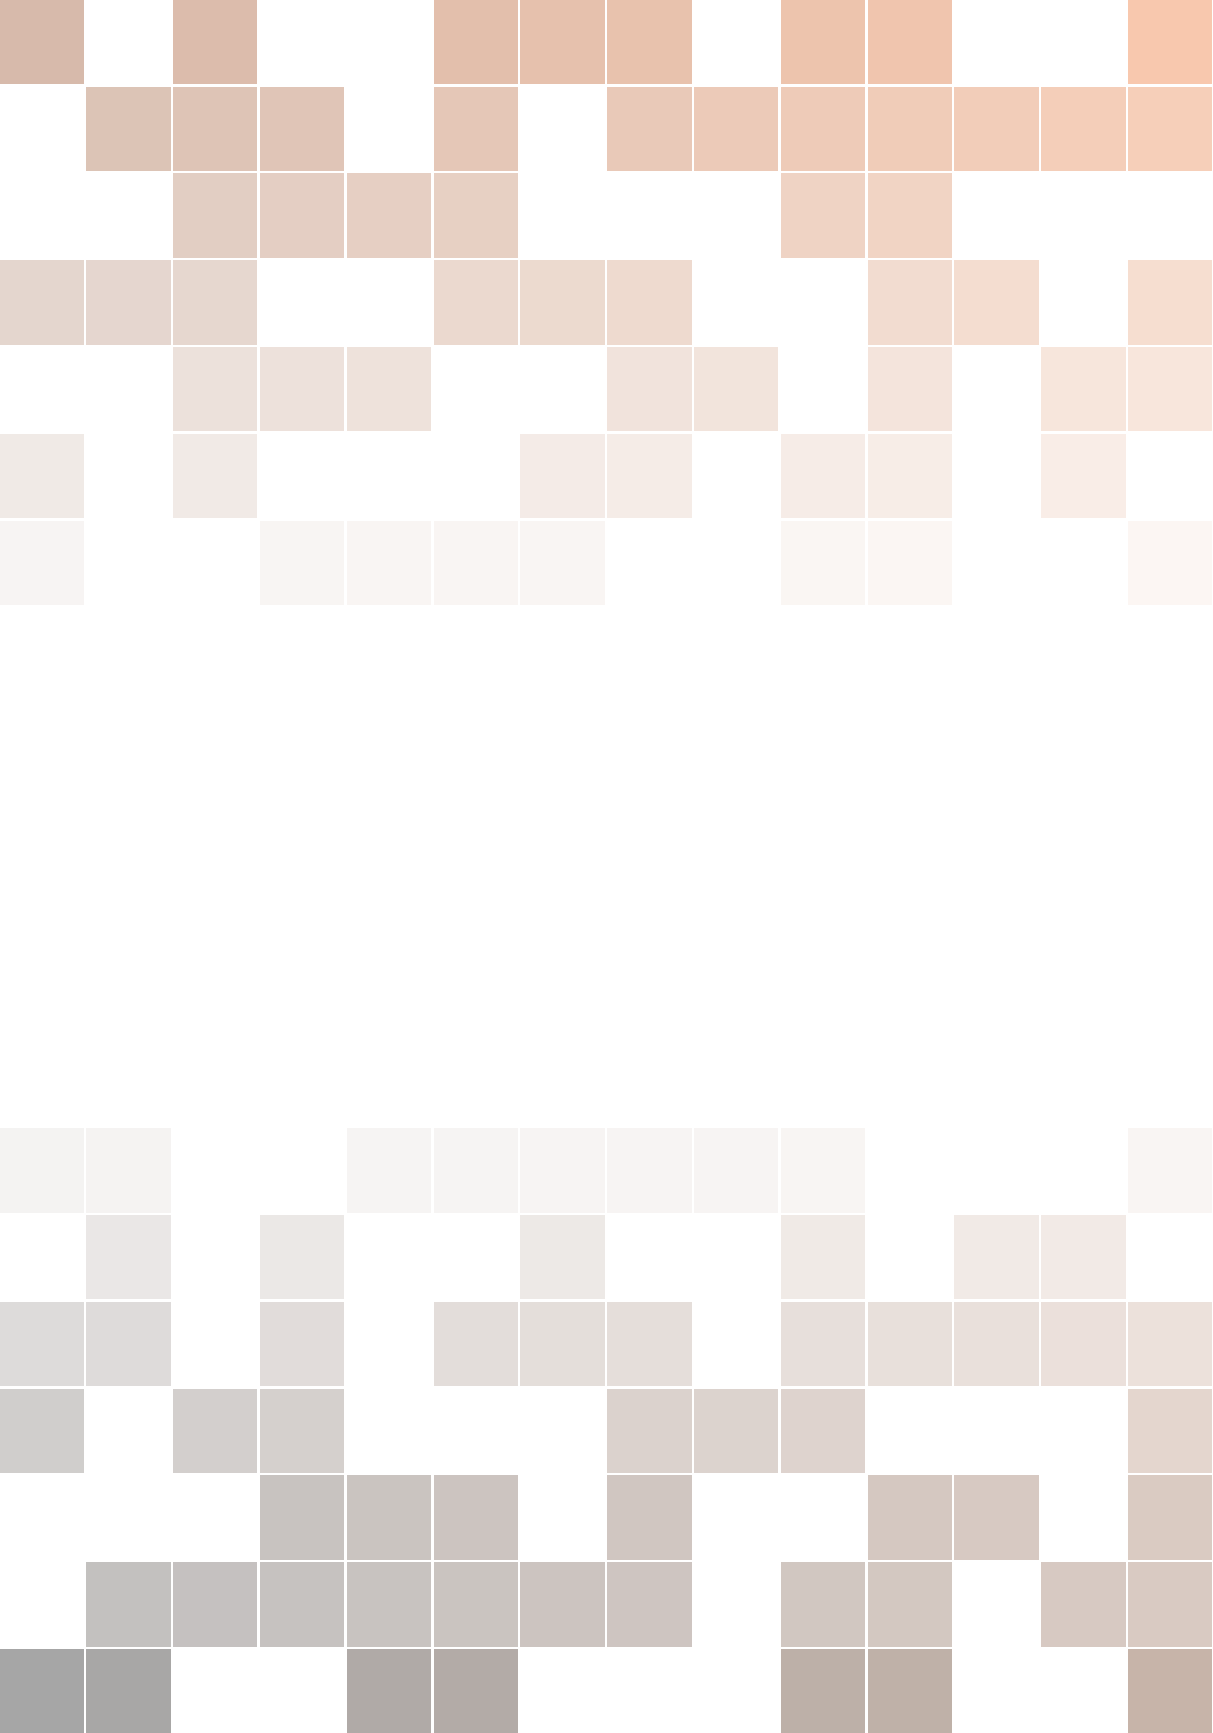
\includegraphics[width=\paperwidth]{background.pdf}};
\draw (current page.center) node [fill=blue!30!white,fill opacity=0.6,text opacity=1,inner %sep=1cm]{\Huge\centering\bfseries\sffamily\parbox[c][][t]{\paperwidth}{\centering Álgebra Linear\\[15pt] % Book title
sep=1cm]{\Huge\centering\bfseries\parbox[c][][t]{\paperwidth}{\centering Curso de Matemática e Tecnologia\\[15pt] % Book title
%{\Large A Profound Subtitle}\\[20pt] % Subtitle
{\huge Prof. Dr. Edson F. Fumachi}}}; % Author name
\end{tikzpicture}
\vfill
\endgroup

%----------------------------------------------------------------------------------------
%	COPYRIGHT PAGE
%----------------------------------------------------------------------------------------
\newpage
~\vfill
\thispagestyle{empty}

\noindent Copyright \copyright\ 2018-2020 E. F. Fumachi\\ % Copyright notice

\noindent \textsc{Material Independente}\\ % Publisher

\noindent \textsc{fumachi.mat.br}\\ % URL

\noindent Licensed under the Creative Commons Attribution-NonCommercial 3.0 Unported License (the ``License''). You may not use this file except in compliance with the License. You may obtain a copy of the License at \url{http://creativecommons.org/licenses/by-nc/3.0}. Unless required by applicable law or agreed to in writing, software distributed under the License is distributed on an \textsc{``as is'' basis, without warranties or conditions of any kind}, either express or implied. See the License for the specific language governing permissions and limitations under the License.\\ % License information, replace this with your own license (if any)

\noindent \textit{Primeira Versão, Janeiro de 2020; Segunda Versão, Maio de 2020; Terceira Versão, Agosto de 2020.} % Printing/edition date
%----------------------------------------------------------------------------------------
%	SYGNATURE PAGE
%----------------------------------------------------------------------------------------
\newpage
\thispagestyle{plain}
%\addcontentsline{toc}{chapter}{\protect\numberline{}Sobre o autor}
\phantomsection
\addcontentsline{toc}{chapter}{\protect\numberline{}Sobre o autor}

%\addvspace{12pt}\Huge\bfseries\textit{Sobre o autor}
\begin{figure}[H]
	\flushright
\includegraphics[width=.2\linewidth]{Pictures/eu01.jpg}
	\label{fig:eu}
\end{figure}
\newcommand*{\tituloautor}{\addvspace{12pt}\Huge\fontfamily{yes}\selectfont}
\newcommand*{\descricaoautor}{\fontfamily{yes}\selectfont}
{\tituloautor\textbf{Sobre o Autor}}
\\
\\
{\descricaoautor{O Prof. Dr. Edson Fernando \textbf{Fumachi} nasceu em Itatiba-SP em 18 de Maio de 1983. Estudou em escolas públicas até o ensino médio. Ingressou no ano 2001 no Curso de Licenciatura em Matemática na Universidade São Francisco, obtendo seu título em 2003. Em 2004 começou a trabalhar no ensino superior da mesma faculdade na qual se graduou. No ano de 2005 assumiu a posição de professor PEB-II do Governo do Estado de São Paulo na disciplina de Matemática. Exonerou do cargo em 2007 para dar sequência no ensino superior. Trabalhou como professor do ensino médio público e privado; no ensino médio privado atuou como professor de Matemática e Física. Em 2007 começou seus estudos como aluno de matéria isolada no Instituto Nacional de Pesquisas Espaciais - INPE, localizado em São José dos Campos-SP. Em 2009 entrou no mesmo instituto como aluno regular do Curso de Mestrado em Engenharia e Tecnologia Espaciais área de concentração em Ciência e Tecnologia dos Materiais e Sensores. Em 2011 defendeu sua Dissertação intitulada \textit{Simulação do fluxo reacional de um reator de filamento quente através da simulação direta de Monte Carlo}. Consecutivamente, em 2011, ingressou no Curso de Doutorado na mesma área do mesmo instituto. Em 2017 defendeu seu Doutorado intitulado \textit{Desenvolvimento de um tubo de queda livre para o modelamento e otimização do processo de solidificação de ligas eutéticas de bismuto-estanho em ambiente de microgravidade}. Tem experiência no meio empresarial através de consultorias realizadas na área de telecomunicações e desenvolvimento de algoritmos para otimização de processos e redução de custos. Tem amplo conhecimento em programação de computadores nas linguagens ForTran77, C e Python. Desenvolve materiais didáticos (como este!) em diversos formatos e linguagens (\LaTeX). Desenvolve conteúdos educacionais e os disponibiliza em plataformas digitais, Youtube e Facebook, sob o pseudônimo Doutor Exatas. }}







%----------------------------------------------------------------------------------------
%	SYGNATURE PAGE
%----------------------------------------------------------------------------------------
\newpage
\thispagestyle{plain}
%\addcontentsline{toc}{chapter}{\protect\numberline{}Sobre o autor}
\phantomsection
\addcontentsline{toc}{chapter}{\protect\numberline{}Prefácio}

\newcommand*{\titulointro}{\addvspace{12pt}\Huge\fontfamily{yes}\selectfont}
\newcommand*{\descricaointro}{\fontfamily{yes}\selectfont}
{\titulointro\textbf{Prefácio}}
\\
\\
{\descricaointro{\indent Este material foi elaborado exclusivamente pelo autor e tem como objetivo atender alunos dos mais variados cursos, Administração, Ciências Contábeis, Tecnólogos, Matemática, Engenharia entre outros. Este material está \textit{\textbf{continuamente em desenvolvimento}} e é distribuído em partes, ou seja, apenas os capítulos necessários aos estudantes de uma determinada disciplina. Portanto, se quiser a versão mais nova e completa, contate o autor enviando um e-mail para \textit{effumachi@gmail.com}. %\cite{flemming2007,hoffmann2008,tan2008,jacques2010,bonafini2011,murolo2011,oliveira2016,barbosa2017,castanheira2017,panonceli2017,souza2018,munaretto2018,boldrini1986,steinbruch2009,franco2016,fernandes2017,domingues2018}.
\vspace{.5cm}

Os exemplos que possuem uma versão em vídeo possuirão o símbolo \video \, e um \textit{link} que encaminhará ao canal do "Doutor Exatas", no Youtube (\url{https://www.youtube.com/channel/UCqGy3MbhdZsWGGBBg7yUGRw}). O leitor pode, ainda, encontrar o conteúdo no Facebook
(\url{https://www.facebook.com/doutorexatas/}).
\vspace{.5cm}

%As ementas das disciplinas de matemática para os cursos de Administração e Ciências Contábeis devem ter elementos fundamentais para desenvolver competências e habilidades dos discentes, deste modo, este livro abordará os seguintes conteúdos:
%\vspace{.5cm}
%\begin{itemize}
%	\item{Revisão sobre conjuntos numéricos e equações de grau 1;}
%	\item{Funções de uma variável real: Domínio, Imagem, funções lineares, quadráticas e seus gráficos;}
%	\item{Limites de funções de uma variável real;}
%	\item{Derivadas de funções, regras e aplicações;}
%	\item{Integrais indefinidas e definidas, cálculo de áreas e aplicações.}
%\end{itemize}
%\vspace{.5cm}

A abordagem adotada neste material é fornecer um pouco de teoria (porém suficiente), e em seguida com a resolução de exemplos.

\vspace{1cm}
Bons estudos.}}
%----------------------------------------------------------------------------------------
%	TABLE OF CONTENTS
%----------------------------------------------------------------------------------------

\usechapterimagefalse % If you don't want to include a chapter image, use this to toggle images off - it can be enabled later with %\usechapterimagetrue
\chapterimage{chapter_head_1.pdf} % Table of contents heading image
\pagestyle{empty} % Disable headers and footers for the following pages
\tableofcontents % Print the table of contents itself
\cleardoublepage % Forces the first chapter to start on an odd page so it's on the right side of the book
\pagestyle{fancy} % Enable headers and footers again

\part{Funções}						% <- Matemática
\chapterimage{chapter_head_2.pdf} % Chapter heading image

\chapter{Revisão sobre conjuntos numéricos e equações}\index{Revisão sobre conjuntos numéricos e equações}
\section{Introdução}\index{Introdução}

O entendimento sobre conjuntos numéricos é fundamental pois através deste conhecimento é possível aplicar corretamente algoritmos e entender suas limitações. Uma situação, muito comum, quando se aplica a matemática em outras ciências é entender o significado daquele resultado obtido no problema real proposto.

\section{Conjuntos numéricos}\index{Conjuntos numéricos}

Os conjuntos numéricos têm aplicações desde tempos remotos e foram desenvolvidos ao longo do tempo para contemplar as possibilidades e soluções de problemas práticos.

Imagine uma situação hipotética na qual um indivíduo possua dezenas de animais por exemplo, dezenas de vacas leiteiras. Um vizinho deste indivíduo também possui dezenas de vacas leiteiras. Ambos compartilham o mesmo local para levarem suas vacas para se alimentarem. Ambos vivem numa época em que não existe um tipo formal de escrita, sequer números! Ao final do dia eles retornam para suas "residências" juntamente com seus animais.

O leitor pode imaginar que em algum momento isso possa gerar alguma confusão, não é? A confusão é que algum dos dois possa ter, ao final do dia, menos ou mais animais que realmente possuíam ao sair pela manhã. Este tipo de problema poderia ter acontecido e precisaria de uma solução.

Talvez, a solução encontrada seja uma espécie de contagem através de comparação. Para cada animal existente em sua casa, haveria uma "pedra". Assim, ao sair pela manhã, cada vaca que deixasse o estaleiro uma pedra seria adicionada a um tipo de bolsa rudimentar que o indivíduo carregaria consigo durante a viagem.

Ao voltar para sua casa, a comparação aconteceria novamente mas de modo inverso, ou seja, para cada vaca que entrasse no estaleiro, uma pedra seria retirada da bolsa. Deste modo, poderiam acontecer 3 situações possíveis, com a quantidade de pedras da bolsa:

\begin{enumerate}
	\item{Sobrar pedras: isso indicaria que algumas vacas não chegaram à sua casa;}
	\item{Faltar pedras: isso indicaria que ele estava com mais vacas, possivelmente sendo alguma de seu vizinho;}
	\item{Não sobrar pedras: todas as vacas que saíram, retornaram e se juntaram no estaleiro.}
\end{enumerate}

Esse processo funcionaria bem, até que o número de animais se tornasse grande o suficiente para ser inviável carregar todas as pedras em sua bolsa. Um sistema de contagem/registro seria interessante!

Desse modo, é possível pensar na aplicabilidade do conjunto dos \textit{Número Naturais}, ou seja, da natureza!

O conjunto dos \textit{Número Naturais}, será definido como segue:

$$
\mathbb{N}=\{1,2,3,\cdots\}
$$

É possível verificar um ponto de divergência em relação a outros autores de livros de matemática: o número 0 (zero) não será definido como número natural pois dificilmente o leitor ouvirá alguém dizendo \textit{"Eu possuo ZERO Ferrari!"} ou algo do tipo \textit{"Eu tenho ZERO reais na carteira!"}.

A evolução continuou a acontecer e a necessidade de novos conjuntos numéricos foram aparecendo. A ideia de números negativos, comum para a atualidade nas relações financeiras, podem ser representados pelo conjunto dos \textit{Números Inteiros} e pode ser definido como:

$$
\mathbb{Z}=\{\cdots ,-2, -1, 0, 1, 2, \cdots\}
$$

Ressalta-se que o número 0 (zero), foi incorporado neste momento no conjunto entretanto, provavelmente ele foi o último algarismo a ser criado. O leitor pode fazer pesquisas adicionais para saber sobre a história do número 0.

Pagamento de impostos sobre terras, construções de prédios, entre outros, levaram a humanidade a desenvolver um novo conjunto de números, os \textit{Números Racionais}:

\begin{ceqn}
\begin{align*}
\mathbb{Q}=\left \{\frac{a}{b} , a \wedge b \in \mathbb{Z}, b \neq 0\right \}
\end{align*}
\end{ceqn}
\\
\indent No entanto, esses números não podiam descrever todas as situações possíveis. Um exemplo disso é o famoso problema proposto por Pitágoras juntamente com seu teorema.
\\

\begin{theorem}[Teorema de Pitágoras]
	Em um triângulo retângulo, a soma dos quadrados dos catetos é igual ao quadrado da hipotenusa.
\end{theorem}


Porém, dado um triângulo retângulo com catetos iguais a 1, tem-se:

\begin{ceqn}
\begin{align*}
c^2 &= a^2 + b^2 \\
c^2 &= 1^2 + 1^2 \\
c^2 &= 1+1 \\
c^2 &= 2 \\
c &= \sqrt{2}
\end{align*}
\end{ceqn}
\\
\indent Neste ponto, começaram os problemas para Pitágoras. Até o momento, não existia solução para descrever o número $\sqrt{2}$. Muito tempo passou e esse tipo de número, os números que não podem ser escritos de modo \textit{Racional}, foram definidos como \textit{Números Irracionais}. Alguns exemplos desses números pode ser visto abaixo:

\begin{ceqn}
	\begin{align*}
	\mathbb{I}=\{\sqrt{2}, \sqrt{3}, \pi, \mathrm{e}, \cdots \}
	\end{align*}
\end{ceqn}
\\
\indent O conjunto dos \textit{Números Irracionais} é infinito!

Assim, tudo parecia estar bem resolvido pois a \textbf{união} entre os \textit{Números Racionais} e \textit{Números Irracionais} foi definido como \textit{Números Reais}.

Mas haveria um tipo de problema que poderia deixar, novamente, os matemáticos com os cabelos em pé. Seja a equação do segundo grau $x^2+4=0$ e calcule as suas raízes:

\begin{ceqn}
	\begin{align}\label{complexo}
	x^2+4&=0 \\ \nonumber
	x^2+4-4&=0-4 \\ \nonumber
	x^2 + 0 &= -4 \\ \nonumber
	x^2 &= -4 \\ \nonumber
	x &= \pm \sqrt{-4} 
	\end{align}
\end{ceqn}
\\
\indent O leitor pode concluir, dependendo de sua formação matemática anterior, que este resultado, simplesmente, não existe. O que está profundamente equivocado!
\\
\indent A solução para este tipo de problema veio através da criação de um conjunto de números chamado \textit{Números Complexos} com a seguinte definição:

\begin{ceqn}
	\begin{align*}
	i = \sqrt{-1}		
	\end{align*}
\end{ceqn}

\indent Enfim, o Problema \ref{complexo} fica:

\begin{ceqn}
	\begin{align*}
	x &= \pm \sqrt{-4} \\
	x &= \pm \sqrt{4 \cdot (-1)} \\
	x &= \pm \sqrt{4} \cdot \sqrt{-1} \\
	x &= \pm 2 \cdot i
	\end{align*}
\end{ceqn}

\indent De modo geral, a definição dos \textit{Números Complexos} é:

\begin{ceqn}
	\begin{align*}
	\mathbb{C} = \left\{ a+bi, a \wedge b \in \mathbb{R}, b\neq 0 \right\}
	\end{align*}
\end{ceqn}


\section{Resolução de equações}\index{Resolução de equações}

\indent O leitor deve ter verificado a resolução do Problema \ref{complexo} que apareceu um $-4$ na resolução. Será explicado os conceitos básicos na resolução deste problema:

\begin{example}
\video \, Calcule a raíz da equação do primeiro grau, $2x+4=10$.
\\
\textbf{\textit{Solução:}}
\\
Calcular a raíz dessa equação, significa determinar o valor de $x$ de modo que a \textit{igualdade} aconteça. Assim, inicia-se o processo copiando a equação dada no enunciado:

\begin{ceqn}
	\begin{align*}
	2x+4=10
	\end{align*}
\end{ceqn}

Para determinar o valor da variável $x$ faz-se necessário isolar a variável em um dos lados da equação. Neste caso, será isolado do lado esquerdo da equação. O leitor pode ter imaginado que seria apenas \textit{passar o 4 para o outro lado com o sinal invertido}, mas se o sinal é de uma \textit{igualdade}, então passar algo de um lado para outro \textit{desequilibraria} a equação e o sinal de $=$ não seria conveniente.
\\
\indent O \textit{\textbf{correto}} é adicionar elementos em \textit{ambos os lados da igualdade}. Neste caso, percebe-se que o número $+4$ está do mesmo lado que a variável, logo ele está \textit{"atrapalhando"}, no entanto, se for adicionado $-4$ em ambos os lados da equação, resultará:

\begin{ceqn}
	\begin{align*}
	2x+4 \textcolor{red}{-4} = 10 \textcolor{red}{-4}
	\end{align*}
\end{ceqn}

A escolha do $-4$ não foi aleatória. No conjunto dos Número Reais, \textit{todo elemento (no caso $+4$) operado (operação $+$ usual) com seu simétrico ($-4$) resulta no elemento neutro ($0$ - zero) da operação ($+$)}, logo:

\begin{ceqn}
	\begin{align*}
	2x + 0 = 6
	\end{align*}
\end{ceqn}

Como visto acima, $0$ é o \textit{elemento neutro da operação de soma}, logo, qualquer elemento operado com o $0$, resultado nele mesmo, assim:

\begin{ceqn}
	\begin{align*}
	2x = 6
	\end{align*}
\end{ceqn}

É popularmente conhecido, neste passo, \textit{"se está multiplicando, então passa dividindo"}, mas acredito que o leitor queira saber o conceito correto, não é mesmo?
A raiz de uma equação está relacionada com o valor de $x$ e não de $2x$, logo, se multiplicar ambos os lados da equação por $\frac{1}{2}$ ter-se-á:

\begin{ceqn}
	\begin{align*}
	\left(\frac{1}{2} \right) \cdot \qquad 2x=6 \qquad \cdot \left(\frac{1}{2} \right)
	\end{align*}
\end{ceqn}

Novamente, o $\frac{1}{2}$ não foi escolhido aleatoriamente, ele foi escolhido por ser o \textit{elemento inverso do $2$}. No conjunto dos números Reais, \textit{todo elemento (no caso, $2$) operado ($\cdot$) com seu inverso ($\frac{1}{2}$) resulta no elemento neutro ($1$) da operação (multiplicação, $\cdot$)}, assim:

\begin{ceqn}
	\begin{align*}
	1 \cdot x = 6 \cdot \frac{1}{2}
	\end{align*}
\end{ceqn}

Como o $1$ é o \textit{elemento neutro da multiplicação}, então $1 \cdot x = x$, logo:

\begin{ceqn}
	\begin{align*}
	x=6 \cdot \frac{1}{2}
	\end{align*}
\end{ceqn}

A multiplicação de frações é feita através da multiplicação entre os \textit{numeradores} e os \textit{denominadores} de cada fração, logo:

\begin{ceqn}
	\begin{align*}
	x = \frac{6}{1} \cdot \frac{1}{2} = \frac{6 \cdot 1}{1 \cdot 2} = \frac{6}{2}
	\end{align*}
\end{ceqn}

Assim, o número que multiplicado por $2$ (denominador) resulta em $6$ (numerador) é o $3$, então:

\begin{ceqn}
	\begin{align*}
	x = 3
	\end{align*}
\end{ceqn}

Para verificar se o resultado obtido está correto basta substituir o valor de $x$ calculado na equação do enunciado, então:

\begin{ceqn}
	\begin{align*}
	2x+4 &= 10 \\
	2 \cdot 3 +4 &= 10 \\
	6+4 &= 10 \\
	10 &= 10 \qquad \mathrm{Verdade!}
	\end{align*}
\end{ceqn}

Assim, $x=3$ é a raíz da equação. É possível representar a solução da equação assim: $\mathrm{S}=\{3\}$.
\\

\doutor \, \url{https://www.youtube.com/watch?v=JY6BJWb1PVY}

\end{example}

Os conceitos abordados no exemplo é de fundamental importância para o entendimento da matemática, tornando-a menos \textit{"complicada"} conforme o leitor avança nos estudos. O leitor poderá ver alguns outros conceitos, tal como regras de sinais (\video) no link \url{https://www.youtube.com/watch?v=IykgcfYnsaQ}.

Todo este material possuirá, como mencionado no Prefácio, uma breve teoria seguido por exemplos resolvidos; com o mesmo nível de detalhamento do exemplo anterior.

\section{Exercícios}\index{Exercícios}

\begin{exercise}
	Faça uma representação gráfica dos conjuntos numéricos.
\end{exercise}

\begin{exercise}
	Resolva a equação $2x-5=0$ considerando os conjuntos:
	\begin{itemize}
		\item[a.]{$\mathbb{N}$}
		\item[b.]{$\mathbb{Z}$}
		\item[c.]{$\mathbb{Q}$}
		\item[d.]{$\mathbb{R}$}
		\item[e.]{$\mathbb{C}$}
	\end{itemize}
\end{exercise}

\begin{exercise}
	Determine os conjuntos Domínio e Imagem para cada uma das funções abaixo:
	\begin{itemize}
		\item[a.]{$3x+4=0$}
		\item[b.]{$f(x) = x^2 + 6$}
		\item[c.]{$f(x) = \frac{1}{x}$}
		\item[d.]{$f(x) = \sqrt{2x}$}
		\item[e.]{$f(x) = \sqrt{-4x}$}
		\item[f.]{$f(x) = \frac{4}{\sqrt{x^2-4}}$}
	\end{itemize}
\end{exercise}

\begin{exercise}
	Determine matematicamente se $f(x) = 3x + 6$ é crescente ou decrescente.
\end{exercise}
\chapterimage{chapter_head_2.pdf} % Chapter heading image

\chapter{Funções}
\section{Introdução}\index{Introdução}


\indent O estudo de funções é importante entretanto, no dia a dia da maior parte das pessoas, este estudo não faz sentido, num primeiro momento. Porém não é difícil imaginar que em toda a vida de uma pessoa ela esteja direta, ou indiretamente, ligada com as funções. Desde a elaboração de uma receita de um bolo, a quilometragem que um determinado veículo pode fazer com um tanque de combustível, a \textit{Receita}, o \textit{Custo} e o \textit{Lucro} de uma empresa.
\\
\indent Considere os ingredientes necessários para se fazer um (uma receita) bolo (hipotético):
\\

\begin{itemize}
	\item{4 ovos;}
	\item{1 litro de leite;}
	\item{1 kg de farinha.}
\end{itemize}
\vspace{.5cm}

Como mencionado, os ingredientes acima estão relacionadas para se fazer \textit{uma receita} ou \textit{um bolo}. Se o indivíduo deseja fazer \textit{duas receitas}, ou \textit{dois bolos}, a quantidade dos ingredientes deve dobrar! Assim:
\\

\begin{itemize}
	\item{4 ovos $\times$ 2 $\Rightarrow$ 8 ovos;}
	\item{1 litro de leite $\times$ 2 $\Rightarrow$ 2 litros de leite;}
	\item{1 kg de farinha $\times$ 2 $\Rightarrow$ 2 kg de farinha.}
\end{itemize}
\vspace{.5cm}

Se uma empresa fabrica um produto por um custo de $\mathrm{R}\$ 10,00$ a unidade e o vende a $\mathrm{R}\$ 15,00$ a unidade e tem custos de aluguel, água, energia elétrica, entre outros que totalizam $\mathrm{R}\$ 1000,00$ por mês é possível escrever sua função \textit{Custo, Receita e Lucro} da seguinte forma:

\begin{ceqn}
	\begin{align*}
	\mathrm{R}(x) &= 15,00 \cdot x \\
	\mathrm{C}(x) &= 10,00 \cdot x +1000,00 \\
	\mathrm{L}(x) &= 5,00 \cdot x -1000,00
	\end{align*}
\end{ceqn}
\vspace{.5cm}
onde $x$ representa a quantidade de itens produzidos e vendidos.

\section{Domínio, imagem, relação e função}\index{Domínio, imagem, relação e função}

Esta seção se inicia com a ideia de \textit{Relação}. A relação deve acontecer entre dois conjuntos numéricos, $\mathbb{A}$ e $\mathbb{B}$, por exemplo.

A \textit{Relação} poderá receber o nome de \textit{Função} se, e somente se, todo elemento do conjunto de partida ($\mathbb{A}$, por exemplo), tenha um, apenas um, correspondente no conjunto de destino ($\mathbb{B}$), através de uma lei. Matematicamente, uma função pode ser escrita assim:

\begin{ceqn}
	\begin{align*}
	f: \mathbb{A} \rightarrow \mathbb{B}, \forall x \in \mathbb{A}, \, \exists y \in \mathbb{B} \,\, / \,\, y=f(x)
	\end{align*}
\end{ceqn}
\\
Vale notar que $x$ é a \textit{variável independente} e $y$ é a \textit{variável dependente} pois depende de $x$. De modo geral, o primeiro conjunto da definição de uma função está relacionado com a \textit{variável independente}, pois é o conjunto de partida e a \textit{variável dependente} está relacionada com o segundo conjunto, pois é o conjunto de chegada.

Como o objetivo deste material é trabalhar com funções, apenas, não será abordado as relações de modo geral, sendo assim deve ser definido o Domínio ($\mathrm{D}$) e Imagem ($\mathrm{Im}$) de uma função ($f$), sendo:

\begin{definition}[Domínio de uma função]
	O domínio de uma função é um conjunto numérico com os valores possíveis que podem ser atribuídos à \textit{variável independente}.
\end{definition}
\vspace{.5cm}
\begin{definition}[Imagem de uma função]
	A imagem de uma função é um conjunto numérico contendo o resultado de cada elemento do domínio aplicado na função.
\end{definition}
\vspace{.5cm}

\begin{example}
	Considere os conjuntos $\mathbb{A}=\{1,2,3\}$ e $\mathbb{B}=\{2,4,6,8\}$ e a função $f: \mathbb{A} \rightarrow \mathbb{B} \,\, / \,\, y=f(x)=2x$. Determine o Domínio e a Imagem de $f$.

\vspace{.5cm}
\textit{\textbf{Solução:}}

\vspace{.5cm}
O conjunto de partida é o conjunto $\mathbb{A}$ então, ele é o \textit{Domínio} da função ($\mathrm{D}(f)$). Os elementos do domínio são atribuídos à \textit{variável independente}, $x$.

Os elementos da \textit{Imagem} da função $f$ são obtidos da seguinte maneira:
\vspace{.5cm}
\begin{itemize}
	\item{$x=1 \Rightarrow f(1)=2\cdot 1 = 2$}
	\item{$x=2 \Rightarrow f(2)=2\cdot 1 = 4$}
	\item{$x=3 \Rightarrow f(3)=2\cdot 1 = 6$}
\end{itemize}

\vspace{.5cm}
Assim, o conjunto \textit{Imagem} é: $\mathrm{Im}=\{2,4,6\}$. Verifica-se que o conjunto imagem não é o conjunto $\mathbb{B}$ pois são os elementos que possuem um elemento $x$ do Domínio. Como o $8$ do conjunto $\mathbb{B}$ não possui um antecessor do conjunto $\mathbb{A}$, ele não faz parte da Imagem.
\end{example}

As funções, de modo geral, tem o conjunto dos \textit{Números Reais} como \textit{Domínio} e \textit{Imagem}, porém existem funções que o Domínio deve ser determinado, ou seja, será um subconjunto dos Reais.

\begin{example}
	Determine o Domínio e a Imagem da função $f(x)=\frac{1}{x-3}$

\vspace{.5cm}
\textit{\textbf{Solução:}}

\textit{Determinação do Domínio}: É possível verificar que a função possui uma divisão e a variável independente está no denominador. Este tipo de situação requer que o \textit{denominador seja diferente de zero}, pois, caso contrário, haveria uma indeterminação. Seguindo o analisado, é possível fazer:

\begin{ceqn}
	\begin{align*}
	x-3 &\neq 0 \\
	x-3 +3 & \neq 0+3 \\
	x &\neq 3
	\end{align*}
\end{ceqn}
Logo, $\mathrm{D}(f)=(-\infty,3) \wedge (3,+\infty)$ ou $\mathrm{D}(f)= \mathbb{R}-\{3\}$ ou $\mathrm{D}(f)=\{x \in \mathbb{R}/ x \neq 3\}$

\vspace{.5cm}
\textit{Determinação da Imagem}: Para a determinação da imagem é necessário analisar os extremos do domínio. Assim:

\vspace{.5cm}
\begin{itemize}
	\item{$x \rightarrow -\infty \Rightarrow f(x) \rightarrow 0$: Se $x$ aproxima-se do infinito negativo, o denominador torna-se um número muito grande e, consequentemente, a divisão aproxima-se de zero;}
	\item{$x \rightarrow -3^{-} \Rightarrow f(x) \rightarrow -\infty$: Se $x$ aproxima-se do três negativo pela esquerda, o denominador torna-se um número muito pequeno negativo e, consequentemente, a divisão aproxima-se de menos infinito;}
	\item{$x \rightarrow -3^{+} \Rightarrow f(x) \rightarrow \infty$: Se $x$ aproxima-se do três negativo pela direita, o denominador torna-se um número muito pequeno positivo e, consequentemente, a divisão aproxima-se de mais infinito;}
	\item{$x \rightarrow \infty \Rightarrow f(x) \rightarrow 0$: Se $x$ aproxima-se do infinito positivo, o denominador torna-se um número muito grande e, consequentemente, a divisão aproxima-se de zero.}
\end{itemize}

\vspace{.5cm}
Do exposto anteriormente, a Imagem nunca assumirá o valor $0$ (zero), assim a imagem será $\mathrm{Im}(f)=\mathbb{R}^{*}$ ou $\mathrm{Im}(f)=\mathbb{R}-\{0\}$
\end{example}

\vspace{.5cm}
Muitos símbolos foram usados no exemplo anterior porém, os mesmos, serão explicados posteriormente no Capítulo \ref{limites}.

\begin{example}
	Determine o Domínio e a Imagem da função $f(x)=\sqrt{x+2}$.

\vspace{.5cm}
\textit{\textbf{Solução:}}

\textit{Domínio}: Os valores que podem ser colocados na função são valores positivos (funções reais) e, nesse caso, o zero. Valores negativos dentro da raíz quadrada resultam em resultados pertencentes aos \textit{Número Complexos}, logo:

\begin{ceqn}
	\begin{align*}
	x+2 & \geq 0 \\
	x+2-2 &\geq 0-2 \\
	x &\geq -2
	\end{align*}
\end{ceqn}

Assim, $\mathrm{D}(f)=[-2,+\infty)$ ou $\mathrm{D}(f)=\{x \in \mathbb{R}/x \geq -2\}$
\end{example}

\section{Raízes de uma função}\index{Raízes de uma função}

As raízes de uma função $f(x)$ pode ser calculada ao fazer $f(x)=0$, ou seja, são os pontos em que a função "corta" o eixo da variável independente. Nos casos de polinômios, o número de raízes é igual ao maior grau da função.
Cada tipo de função possui uma metodologia diferente para o cálculo das suas raízes assim, será visto nas seções subsequentes.

\section{Funções de uma variável real}\index{Funções de uma variável real}

Difíceis são os processos que dependem apenas de uma variável, ou seja, ao estudar o consumo de combustível de um veículo não pode ser pensado somente na qualidade do combustível, mas deve ser pensado na alinhamento e pressão dos pneus, da temperatura, das condições da rodovia, das manutenções, da qualidade do óleo do motor, do modo como o veículo é conduzido (esta variável bem estudada resulta em economia de 30\% no consumo de combustível), entre outros fatores.

Como visto na seção anterior, "geralmente" se atribui $x$ a \textit{variável independente} e $y$ ou $f(x)$ a \textit{variável dependente}, assim, tem-se duas variáveis. Mas como é possível ter duas variáveis sendo que a seção trata de \textit{funções de uma variável}?

A resposta é simples: Funções de uma variável é o nome dado às funções que possuem uma, e apenas uma, \textit{variável independente}.

\begin{example}
	A área do quadrado pode ser representada por uma função de uma variável. Como a área do quadrado é a multiplicação dos dois lados, e os quatro lados são iguais, então:
	
	\begin{ceqn}
		\begin{align*}
		A_Q(l)=l \cdot l = l^2
		\end{align*}
	\end{ceqn}

onde $l$ é a medida do lado do quadrado.
\end{example}

\begin{example}
	A área de um retângulo é uma função de duas variáveis, pois sua área é a multiplicação de dois lados consecutivos. Como os lados do retângulo são iguais aos seus lados opostos, e não necessariamente precisam ter os quatro lados iguais, então:
	
	\begin{ceqn}
		\begin{align*}
		A_R(a,b)=a \cdot b
		\end{align*}
	\end{ceqn}

onde $a$ e $b$ são as medidas dos lados de um retângulo.
\end{example}

\vspace{.5cm}


\section{Funções lineares}\index{Funções lineares}


As \textit{funções lineares} ou \textit{funções do primeiro grau} ou \textit{funções de grau um} são funções do tipo:

\begin{ceqn}
	\begin{align*}
	f(x) = ax +b
	\end{align*}
\end{ceqn}

\vspace{.5cm}
Onde:
\begin{itemize}
	\item{$f$: nome da função;}
	\item{$x$: variável independente;}
	\item{$f(x)$: variável dependente;}
	\item{$a$: coeficiente angular;}
	\item{$b$: coeficiente linear.}
\end{itemize}

\vspace{.5cm}

Um ponto importante para observar é o coeficiente angular. Este valor permite identificar se a função é \textit{crescente} ($a>0$) ou \textit{decrescente} ($a<0$). Caso $a=0$, tem-se uma função constante igual a $f(x)=b$, ou seja, para funções do primeiro grau a condição é que ($a \ne 0$)

De modo geral, uma função $f(x)$ é crescente quando para quaisquer dois valores $x_1$ e $x_2$ pertencentes ao $\mathrm{Dom}(f)$, se $x_2 > x_1$, então $f(x_2)>f(x_1)$. Se $x_2>x_1 \Rightarrow f(x_2)<f(x_1)$ então a função será decrescente.


\begin{example} Determine se a função $f(x)=2x+4$ é crescente ou decrescente.

\textit{\textbf{Solução:}}

	É possível verificar que o coeficiente angular é igual a $2$ e é maior do que zero, no entanto, tomando $x_1=0$ e $x_2=2$ tem-se $f(x_1)=f(0)=2\cdot0+4=4$ e $f(x_2)=f(2)=2\cdot2+4=8$, assim, $x_2>x_1\Rightarrow f(x_2)>f(x_1)$ logo, $f(x)$ é crescente.

\end{example}

\begin{example} Determine se a função $f(x)=-x+4$ é crescente ou decrescente.
	
	\textit{\textbf{Solução:}}
	
	É possível verificar que o coeficiente angular é igual a $-1$ e é menor do que zero, no entanto, tomando $x_1=0$ e $x_2=2$ tem-se $f(x_1)=f(0)=-1\cdot0+4=4$ e $f(x_2)=f(2)=-1\cdot2+4=2$, assim, $x_2>x_1\Rightarrow f(x_2)<f(x_1)$ logo, $f(x)$ é decrescente.
	
\end{example}

\section{Raíz de funções lineares}\index{Raíz de funções lineares}

Como mencionado anteriormente, para determinar a raíz de um função é necessário fazer $f(x)=0$. Como o maior grau das funções lineares é igual a "um" então, ter-se-á, apenas, uma raíz.

\begin{example} Calcule a raíz da função $f(x)=-x+4$
	
	\textit{\textbf{Solução:}}
	
	Fazendo $f(x)=0$, tem-se:
	\begin{ceqn}
		\begin{align*}
		f(x)&=0 \\
		-x+4&=0 \\
		-x+4-4&=0-4 \\
		(-1) \cdot \,\,\,\, -x&=-4\,\,\,\, \cdot (-1) \\
		x&=4
		\end{align*}
	\end{ceqn}
	
	Assim, $x=4$ é a raíz da função $f(x)=-x+4$.
\end{example}

\section{Gráficos de funções lineares}\index{Gráficos de funções lineares}

Em construção

\section{Funções quadráticas}\index{Funções quadráticas}

As \textit{funções quadráticas} ou \textit{funções do segundo grau} ou \textit{funções de grau dois} são funções do tipo:

\begin{ceqn}
	\begin{align*}
	f(x) = ax^2 +bx+c
	\end{align*}
\end{ceqn}

\vspace{.5cm}
Onde:
\begin{itemize}
	\item{$f$: nome da função;}
	\item{$x$: variável independente;}
	\item{$f(x)$: variável dependente;}
	\item{$a$, $b$ e $c$: são coeficientes.}
\end{itemize}

\vspace{.5cm}

Um ponto importante para observar é o coeficiente $a$. Este valor permite identificar se a função possui \textit{concavidade para cima} ($a>0$) ou \textit{concavidade para baixo} ($a<0$). Caso $a=0$, tem-se uma função linear igual a $f(x)=bx+c$, ou seja, para funções do segundo grau a condição é que ($a \ne 0$).

\section{Raízes de funções quadráticas}\index{Raízes de funções quadráticas}

Para o caso de funções do segundo grau, as raízes podem ser calculadas através da, tão conhecida, fórmula de Bháskara, que é:

\begin{ceqn}
	\begin{align*}
	x = \frac{-b \pm \sqrt{b^2-4\cdot a \cdot c}}{2\cdot a}
	\end{align*}
\end{ceqn}

O termo dentro da raíz quadrada, $b^2-4ac$, é conhecido como delta $\Delta$.

\begin{example}\label{caso1}
	Calcule a raíz da função $f(x)=x^2-5x+6$
	
	\textit{\textbf{Solução:}}
	
	Fazendo $f(x)=0$, tem-se:
	\begin{ceqn}
		\begin{align*}
		f(x)&=0 \\
		x^2-5x+6&=0 \\
		\end{align*}
	\end{ceqn}
	
	O próximo passo é identificar os valores dos coeficientes $a$, $b$ e $c$. Para a equação acima, tem-se:
	
	\begin{ceqn}
		\begin{align*}
		a=1 \,\,\,\, b=-5 \,\,\,\, c=6
		\end{align*}
	\end{ceqn}

Determinado os valores dos coeficientes, calcula-se o valor de $\Delta$:
	
	\begin{ceqn}
		\begin{align*}
		\Delta &= b^2-4ac \\
		&=(-5)^2-4 \cdot 1 \cdot 6 \\
		&= (-5)\cdot (-5)-24 \\
		&= 25 - 24 \\
		\Delta &=1 \,\,\,\,\,\,\,\,\,\,\,\,\,\,\,\,\, (\mathrm{Caso 1:}\,\, \Delta>0)
		\end{align*}
	\end{ceqn}
	
	Nesta parte, deverá ser substituído os valores dos coeficientes e o $\Delta$ calculado:
	
	\begin{ceqn}
		\begin{align*}
		x &= \frac{-b\pm \sqrt{\Delta}}{2a} \\
		&= \frac{-(-5)\pm\sqrt{1}}{2\cdot 1} \\
		&= \frac{5 \pm 1}{2} \Rightarrow \\
		x_1 &= \frac{5+1}{2}=\frac{6}{2} \Rightarrow x_1 = 3 \\
		x_2 &= \frac{5-1}{2}=\frac{4}{2} \Rightarrow x_2 = 2 
		\end{align*}
	\end{ceqn}

Assim, as raízes podem ser representadas através do conjunto solução $\mathbb{S}=\{2,3\}$

\end{example}

\begin{example}\label{caso2}
	Calcule a raíz da função $f(x)=x^2-4x+4$
	
	\textit{\textbf{Solução:}}
	
	Fazendo $f(x)=0$, tem-se:
	\begin{ceqn}
		\begin{align*}
		f(x)&=0 \\
		x^2-4x+4&=0 \\
		\end{align*}
	\end{ceqn}
	
	O próximo passo é identificar os valores dos coeficientes $a$, $b$ e $c$. Para a equação acima, tem-se:
	
	\begin{ceqn}
		\begin{align*}
		a=1 \,\,\,\, b=-4 \,\,\,\, c=4
		\end{align*}
	\end{ceqn}
	
	Determinado os valores dos coeficientes, calcula-se o valor de $\Delta$:
	
	\begin{ceqn}
		\begin{align*}
		\Delta &= b^2-4ac \\
		&=(-4)^2-4 \cdot 1 \cdot 4 \\
		&= (-4)\cdot (-4)-16 \\
		&= 16-16 \\
		\Delta &=0 \,\,\,\,\,\,\,\,\,\,\,\,\,\,\,\,\, (\mathrm{Caso 2:}\,\, \Delta=0)
		\end{align*}
	\end{ceqn}
	
	Nesta parte, deverá ser substituído os valores dos coeficientes e o $\Delta$ calculado:
	
	\begin{ceqn}
		\begin{align*}
		x &= \frac{-b\pm \sqrt{\Delta}}{2a} \\
		&= \frac{-(-4)\pm\sqrt{0}}{2\cdot 1} \\
		&= \frac{4 \pm 0}{2} \Rightarrow \\
		x_1 &= \frac{4+0}{2}=\frac{4}{2} \Rightarrow x_1 = 2 \\
		x_2 &= \frac{4-0}{2}=\frac{4}{2} \Rightarrow x_2 = 2 
		\end{align*}
	\end{ceqn}
	
	Assim, as raízes podem ser representadas através do conjunto solução $\mathbb{S}=\{2\}$
	
\end{example}

\begin{example}\label{caso3} Calcule a raíz da função $f(x)=x^2-6x+13$
	
	\textit{\textbf{Solução:}}
	
	Fazendo $f(x)=0$, tem-se:
	\begin{ceqn}
		\begin{align*}
		f(x)&=0 \\
		x^2-6x+13&=0 \\
		\end{align*}
	\end{ceqn}
	
	O próximo passo é identificar os valores dos coeficientes $a$, $b$ e $c$. Para a equação acima, tem-se:
	
	\begin{ceqn}
		\begin{align*}
		a=1 \,\,\,\, b=-6 \,\,\,\, c=13
		\end{align*}		
	\end{ceqn}
	
	Determinado os valores dos coeficientes, calcula-se o valor de $\Delta$:
	
	\begin{ceqn}
		\begin{align*}
		\Delta &= b^2-4ac \\
		&=(-6)^2-4 \cdot 1 \cdot 13 \\
		&= (-6)\cdot (-6)-52 \\
		&= 36 - 52 \\
		\Delta &=-16 \,\,\,\,\,\,\,\,\,\,\,\,\,\,\,\,\, (\mathrm{Caso 3:}\,\, \Delta<0)
		\end{align*}
	\end{ceqn}
	
	Nesta parte, deverá ser substituído os valores dos coeficientes e o $\Delta$ calculado:
	
	\begin{ceqn}
	\begin{align*}
	x &= \frac{-b\pm \sqrt{\Delta}}{2a} \\
	&= \frac{-(-6)\pm \sqrt{-16}}{2\cdot 1} \xRightarrow{\text{\ref{complexo}}} \\
	&= \frac{6 \pm \sqrt{16 \cdot (-1)}}{2} \\
	&= \frac{6\pm \sqrt{16} \cdot \sqrt{-1}}{2} \\
	&= \frac{6\pm 4 \cdot i}{2} \Rightarrow \\
	x_1 &= \frac{6+4i}{2} = 3+2i \\
	x_2 &= \frac{6-4i}{2} = 3-2i \\
	\end{align*}
\end{ceqn}

	Assim, as raízes podem ser representadas através do conjunto solução $\mathbb{S}=\{3 \pm 2i\}$
	
\end{example}

\section{Gráficos de funções quadráticas}\index{Gráficos de funções quadráticas}

Os gráficos de funções de segunda grau podem apresentar 6 formas diferentes, que são:

\begin{itemize}
	\item{Caso 1: $a > 0$ e $\Delta > 0 \Rightarrow$ Parábola com concavidade para \textbf{cima} e duas \textbf{raízes reais distintas};}
	\item{Caso 2: $a > 0$ e $\Delta = 0 \Rightarrow$ Parábola com concavidade para \textbf{cima} e duas \textbf{raízes reais iguais};}
	\item{Caso 3: $a > 0$ e $\Delta < 0 \Rightarrow$ Parábola com concavidade para \textbf{cima} e duas \textbf{raízes complexas};}
	\item{Caso 4: $a < 0$ e $\Delta > 0 \Rightarrow$ Parábola com concavidade para \textbf{baixo} e duas \textbf{raízes reais distintas};}
	\item{Caso 5: $a < 0$ e $\Delta = 0 \Rightarrow$ Parábola com concavidade para \textbf{baixo} e duas \textbf{raízes reais iguais};}
	\item{Caso 6: $a < 0$ e $\Delta < 0 \Rightarrow$ Parábola com concavidade para \textbf{baixo} e duas \textbf{raízes complexas};} \\
\end{itemize}

Para fazer o gráfico é ncessário conhecer alguns pontos fundamentais da função: \\

\begin{itemize}
	\item[1.]{\textbf{Raízes}: Todas as funções do segundo grau possuem raízes, no entanto, as raízes complexas não podem ser representadas no plano real;}
	\item[2.]{\textbf{Vértice}: Todas as funções do segundo grau possuem vértices. Os vértices nessas funções representam um ponto de \textbf{extremo}, que pode ser \textbf{máximo} ($a<0$) ou \textbf{mínimo} ($a>0$);}
	\item[3.]{\textbf{Intercepto com o eixo vertical}: Este valor implica onde a função \textit{"corta o eixo y"}.} \\
\end{itemize}

\begin{example}
	(Caso 1) Determine o gráfico da função $f(x)=x^2-5x+6$
	
	\solucao
	
	Essa função é a mesma do Exemplo \ref{caso1}, ou seja, as raízes já foram determinadas ($x_1 = 2$ e $x_2 = 3$), bem como o valor do $\Delta$ ($= 1$).\\
	
	Assim, é necessário determinar o Vértice. A determinação do mesmo pode ser feita usando:
	
	\begin{ceqn}
		\begin{align*}
		x_v &= \frac{-b}{2a} \Rightarrow x_v = \frac{-(-5)}{2 \cdot 1} = \frac{5}{2} \\
		y_v &= \frac{-\Delta}{4a} \Rightarrow y_v = \frac{-1}{4 \cdot 1} = \frac{-1}{4} \\
		\end{align*}
	\end{ceqn}
	
	Portanto, as coordenadas do Vértice são $\left (\frac{5}{2},\frac{-1}{4} \right )$.\footnote{Um modo mais fácil de representar no plano é usar a representação decimal assim, as coordenadas do vértice ficará $(2,5;-0,25)$.}\\
	
	O último passo é verificar o intercepto com o eixo vertical, ou seja, determinar o valor de $f(x)$ quando $x=0$, assim:
	
	\begin{ceqn}
		\begin{align*}
		f(x) &= x^2-5x+6 \\
		x=0 \Rightarrow f(0)&=0^2-5 \cdot 0 +6 \\
		f(0) &= 6 
		\end{align*}
	\end{ceqn}
	
	Unindo as informações:\\
	\begin{itemize}
		\item[1.]{\textbf{Raízes}: $x_1=(2,0)$ e $x_2=(3,0)$}
		\item[2.]{\textbf{Vértice}:$\left( \frac{5}{2},\frac{-1}{4} \right)$}
		\item[3.]{\textbf{Intercepto}: $(0,6)$}\\
	\end{itemize}
	
	O gráfico fica:\\
	\begin{center}
		\begin{tikzpicture}[scale=1.0,line cap=round,line join=round,>=triangle 45,x=1cm,y=1cm]
		\begin{axis}[
		x=1cm,y=1cm,
		axis lines=middle,
		grid style=dashed,
		ymajorgrids=true,
		xmajorgrids=true,
		xmin=-1.1,
		xmax=6.1,
		ymin=-1.2,
		ymax=7.5,
		xlabel=$x$,
		ylabel=$y$,
		width=10cm,
		xtick={-1,...,6},
		ytick={-1,...,7},]
		\draw[line width=2pt,color=red,smooth,samples=100,domain=-.25:5.25] plot(\x,{(\x)^(2)-5*(\x)+6});
		\begin{scriptsize}
		\draw[color=red] (5.65,6.5) node {$f(x)$};
		\draw[color=black] (2.1,0.3) node {$x_1$};
		\draw[color=black] (3,-0.7) node {Vértice};
		\draw[color=black] (3.1,0.3) node {$x_2$};
		\draw[color=black] (.5,6) node {$f(0)$};
		\end{scriptsize}
		\node [fill=black, circle, scale=0.5] at (axis cs: 0,6) {};
		\node [fill=black, circle, scale=0.5] at (axis cs: 2.5,-.25) {};
		\node [fill=black, circle, scale=0.5] at (axis cs: 2,0) {};
		\node [fill=black, circle, scale=0.5] at (axis cs: 3,0) {};
		\end{axis}
		\end{tikzpicture}
	\end{center}
	
\end{example}
\begin{example}
	(Caso 2) Determine o gráfico da função $f(x)=x^2-4x+4$
	
	\solucao
	
	Essa função é a mesma do Exemplo \ref{caso2}, ou seja, as raízes já foram determinadas ($x_1 =x_2= 2$), bem como o valor do $\Delta$ ($= 0$).\\
	
	Assim, é necessário determinar o Vértice (V). A determinação do mesmo pode ser feita usando:
	
	\begin{ceqn}
		\begin{align*}
		x_v &= \frac{-b}{2a} \Rightarrow x_v = \frac{-(-4)}{2 \cdot 1} = \frac{4}{2}=2 \\
		y_v &= \frac{-\Delta}{4a} \Rightarrow y_v = \frac{-0}{4 \cdot 1} = 0 \\
		\end{align*}
	\end{ceqn}
	
	Portanto, as coordenadas de V são $\left ( 2,0 \right )$.\\
	
	O último passo é verificar o intercepto com o eixo vertical, ou seja, determinar o valor de $f(x)$ quando $x=0$, assim:
	
	\begin{ceqn}
		\begin{align*}
		f(x) &= x^2-4x+4 \\
		x=0 \Rightarrow f(0)&=0^2-4 \cdot 0 +4 \\
		f(0) &= 4\\ 
		\end{align*}
	\end{ceqn}
	
	Unindo as informações:\\
	\begin{itemize}
		\item[1.]{\textbf{Raízes}: $x_1=x_2=(2,0)$}
		\item[2.]{\textbf{Vértice}: $(2,0)$}
		\item[3.]{\textbf{Intercepto}: $(0,4)$}\\
	\end{itemize}
	Das informações anteriores, é possível verificar que as raízes ($x_1$ e $x_2$) têm a mesma coordenada que V, ou seja, $(2,0)$. O processo, nesse caso, fica um pouco complicado pois, na realidade, existem dois pontos apenas: o intercepto e o ponto $(2,0)$.\\
	
	Para resolver esse problema, deve ser escolhido dois valores para $x$, calcular suas imagens ($f(x)$) e usá-los como complemento\footnote{Sugestão: sabendo o $x_v$, neste exemplo $x_v=2$, escolhe-se dois valores para $x$ ($x_3$ e $x_4$, por exemplo), de modo que $|x_v-x_3|=|x_v-x_4|$. Essa escolha baseia-se no fato de que, pelo vértice é possível imaginar um \textit{eixo de simetria}.}. Assim, escolhendo $x_3=1$ e $x_4=3$, tem-se:
	
	\begin{ceqn}
		\begin{align*}
		x_3=1 \Rightarrow f(1) &= 1^2-4 \cdot 1 +4 = 1 \\
		x_4=3 \Rightarrow f(3) &= 3^2-4 \cdot 3 +4 = 1 \\
		\end{align*}
	\end{ceqn}
	
	É possível chamar essas coordenadas calculadas, de pontos, $A$ e $B$, sendo assim, $A=(1,1)$ e $B=(3,1)$
	
	Logo, o gráfico fica:\\
	\begin{center}
		\begin{tikzpicture}[scale=1.4,line cap=round,line join=round,>=triangle 45,x=1cm,y=1cm]
		\begin{axis}[
		x=1cm,y=1cm,
		axis lines=middle,
		grid style=dashed,
		ymajorgrids=true,
		xmajorgrids=true,
		xmin=-0.5,
		xmax=4.6000000000000005,
		ymin=-0.5000013006060611,
		ymax=4.9,
		xlabel=$x$,
		ylabel=$y$,
		width=10cm,
		xtick={-1,0,...,5},
		ytick={-1,0,...,5},]
		\draw[line width=2pt,color=red,smooth,samples=100,domain=-0.1:4.1] plot(\x,{(\x)^(2)-4*(\x)+4});
		\begin{scriptsize}
		\draw[color=red] (3.35,4.2) node {$f(x)$};
		\draw[color=black] (.5,4) node {$f(0)$};
		\end{scriptsize}
		\node [fill=black, circle, scale=0.5] at (axis cs: 0,4) {};
		\node [fill=black, circle, scale=0.5] at (axis cs: 1,1) {};
		\node [fill=black, circle, scale=0.5, pin=75:{A}] at (axis cs: 1,1) {};
		\node [fill=black, circle, scale=0.5, pin=105:{B}] at (axis cs: 3,1) {};
		\node [fill=black, circle, scale=0.1, pin=60:{$x_2$}] at (axis cs: 2,0) {};
		\node [fill=black, circle, scale=0.1, pin=120:{$x_1$}] at (axis cs: 2,0) {};
		\node [fill=black, circle, scale=0.5, pin=90:{V}] at (axis cs: 2,0) {};
		\node [fill=black, circle, scale=0.5] at (axis cs: 3,1) {};
		\end{axis}
		\end{tikzpicture}
	\end{center}
	
\end{example}

\begin{example}
	(Caso 3) Determine o gráfico da função $f(x)=x^2-6x+13$
	
	\solucao
	
	Essa função é a mesma do Exemplo \ref{caso3}, ou seja, as raízes já foram determinadas ($x_1 = 3-2i$ e $x_2 = 3+2i$), bem como o valor do $\Delta$ ($= -16$).\\
	
	A determinação do vértice pode ser feita usando:
	
	\begin{ceqn}
		\begin{align*}
		x_v &= \frac{-b}{2a} \Rightarrow x_v = \frac{-(-6)}{2 \cdot 1} = \frac{6}{2} = 3 \\
		y_v &= \frac{-\Delta}{4a} \Rightarrow y_v = \frac{-(-16)}{4 \cdot 1} = \frac{16}{4}=4 \\
		\end{align*}
	\end{ceqn}
	
	Portanto, as coordenadas do Vértice são $(3,4))$.\\
	
	O último passo é verificar o intercepto com o eixo vertical, ou seja, determinar o valor de $f(x)$ quando $x=0$, assim:
	
	\begin{ceqn}
		\begin{align*}
		f(x) &= x^2-6x+13 \\
		x=0 \Rightarrow f(0)&=0^2-6 \cdot 0 +13 \\
		f(0) &= 13 
		\end{align*}
	\end{ceqn}
	
	Unindo as informações:\\
	\begin{itemize}
		\item[1.]{\textbf{Raízes}: $x_1=3-2i$ e $x_2=3+2i$}
		\item[2.]{\textbf{Vértice}: $(3,4)$}
		\item[3.]{\textbf{Intercepto}: $(0,13)$}\\
	\end{itemize}
	Das informações anteriores, é possível verificar que as raízes ($x_1$ e $x_2$) pertencem aos conjunto dos números complexos e não tem representação no plano real. O processo, nesse caso, fica um pouco complicado pois, na realidade, existem dois pontos apenas: o intercepto e o vértice $(3,4)$.\\
	
	Para resolver esse problema, deve ser escolhido dois valores para $x$, calcular suas imagens ($f(x)$) e usá-los como complemento. Assim, escolhendo $x_3=2$ e $x_4=4$, tem-se:
	
	\begin{ceqn}
		\begin{align*}
		x_3=2 \Rightarrow f(2) &= 2^2-6 \cdot 2 +13 = 5 \\
		x_4=4 \Rightarrow f(4) &= 4^2-6 \cdot 4 +13 = 5 \\
		\end{align*}
	\end{ceqn}
	
	É possível chamar essas coordenadas calculadas, de pontos, $A$ e $B$, sendo assim, $A=(2,5)$ e $B=(4,5)$
	
	O gráfico fica:\\
	\begin{center}
		\begin{tikzpicture}[line cap=round,line join=round,>=triangle 45,x=1.5cm,y=.9cm]
		\begin{axis}[
		x=1.5cm,y=.9cm,
		axis lines=middle,
		grid style=dashed,
		ymajorgrids=true,
		xmajorgrids=true,
		xmin=-1.2,
		xmax=6.9,
		ymin=-1.1,
		ymax=15.,
		xlabel=$x$,
		ylabel=$y$,
		width=10cm,
		xtick={-1,0,...,7},
		ytick={-1,0,...,14},]
		\draw[line width=2pt,color=red,smooth,samples=100,domain=-.25:6.5] plot(\x,{(\x)^(2)-6*(\x)+13});
		\node [fill=black, circle, scale=0.5, pin=45:{$f(0)$}] at (axis cs: 0,13) {};
		\node [fill=black, circle, scale=0.5, pin=75:{A}] at (axis cs: 2,5) {};
		\node [fill=black, circle, scale=0.5, pin=105:{B}] at (axis cs: 4,5) {};
		\node [fill=black, circle, scale=0.5, pin=-45:{V}] at (axis cs: 3,4) {};
		\end{axis}
		\end{tikzpicture}
	\end{center}
	
\end{example}

Os casos em que o valor de $a$ forem menores que zero, o processo é semelhante, no entanto, o resultado será uma parábola com a \textbf{concavidade para baixo}.

\section{Exercícios}\index{Exercícios}

\begin{exercise}
	Qual a diferença entre Equação e Função?
\end{exercise}

\begin{exercise}
	Resolva a equação $x^2+4=0$ considerando os conjuntos:
	\begin{itemize}
		\item[a.]{$\mathbb{N}$}
		\item[b.]{$\mathbb{Z}$}
		\item[c.]{$\mathbb{Q}$}
		\item[d.]{$\mathbb{R}$}
		\item[e.]{$\mathbb{C}$}
	\end{itemize}
\end{exercise}

\begin{exercise}
	Calcule as raízes das funções abaixo e represente graficamente.
	\begin{itemize}
		\item[a.]{$f(x) = 3x - 6$}
		\item[b.]{$g(x) = x^2-5x+6$}
		\item[c.]{$f(y) = 5x - 2$}
		\item[d.]{$f(x) = x^2-4x+4$}
		\item[e.]{$g(w) = w^2+4$}
	\end{itemize}
\end{exercise}
\section{Exercícios}\index{Exercícios}

\begin{exercise}
	Faça uma representação gráfica dos conjuntos numéricos.
\end{exercise}

\begin{exercise}
	Qual a diferença entre Equação e Função?
\end{exercise}

\begin{exercise}
	Resolva a equação $2x-5=0$ considerando os conjuntos:
	\begin{itemize}
		\item[a.]{$\mathbb{N}$}
		\item[b.]{$\mathbb{Z}$}
		\item[c.]{$\mathbb{Q}$}
		\item[d.]{$\mathbb{R}$}
		\item[e.]{$\mathbb{C}$}
	\end{itemize}
\end{exercise}

\begin{exercise}
	Resolva a equação $x^2+4=0$ considerando os conjuntos:
	\begin{itemize}
		\item[a.]{$\mathbb{N}$}
		\item[b.]{$\mathbb{Z}$}
		\item[c.]{$\mathbb{Q}$}
		\item[d.]{$\mathbb{R}$}
		\item[e.]{$\mathbb{C}$}
	\end{itemize}
\end{exercise}

\begin{exercise}
	Determine os conjuntos Domínio e Imagem para cada uma das funções abaixo:
	\begin{itemize}
		\item[a.]{$3x+4=0$}
		\item[b.]{$f(x) = x^2 + 6$}
		\item[c.]{$f(x) = \frac{1}{x}$}
		\item[d.]{$f(x) = \sqrt{2x}$}
		\item[e.]{$f(x) = \sqrt{-4x}$}
		\item[f.]{$f(x) = \frac{4}{\sqrt{x^2-4}}$}
	\end{itemize}
\end{exercise}

\begin{exercise}
	Determine matematicamente se $f(x) = 3x + 6$ é crescente ou decrescente.
\end{exercise}

\begin{exercise}
	Calcule as raízes das funções abaixo e represente graficamente.
	\begin{itemize}
		\item[a.]{$f(x) = 3x - 6$}
		\item[b.]{$g(x) = x^2-5x+6$}
		\item[c.]{$f(y) = 5x - 2$}
		\item[d.]{$f(x) = x^2-4x+4$}
		\item[e.]{$g(w) = w^2+4$}
	\end{itemize}
\end{exercise}
%\part{Cálculo}				% Cálculo
%\chapterimage{chapter_head_2.pdf} % Chapter heading image

\chapter{Limites de funções de uma variável}\label{limites}
\section{Conceito de limite}\index{Conceito de limite}
\section{Limites de funções polinomiais}\index{Limites de funções polinomiais}
\section{Continuidade de funções}\index{Continuidade de funções}

%\chapterimage{chapter_head_2.pdf} % Chapter heading image

\chapter{Derivadas de funções de uma variável}
\section{Taxa de variação}\index{Taxa de variação}
\section{Interpretação geométrica}\index{Interpretação geométrica}
\section{Regras de derivação}\index{Regras de derivação}
\subsection{Função constante}\index{Função constante}
\subsection{Função polinomial}\index{Função polinomial}
\subsection{Função exponencial}\index{Função exponencial}
\subsection{Função logarítmica}\index{Função logarítmica}
\subsection{Produto}\index{Função Produto}
\subsection{Quociente}\index{Quociente}
\subsection{Cadeia}\index{Cadeia}
%\chapterimage{chapter_head_2.pdf} % Chapter heading image

\chapter{Integrais}
\section{Somas infinitas}\index{Somas infinitas}
\section{Integrais indefinidas}\index{Integrais indefinidas}
\section{Integrais definidas}\index{Integrais definidas}
\section{Cálculo de áreas}\index{Cálculo de áreas}
\section{Aplicações das integrais na Administração}\index{Aplicações das integrais na Administração}
\part{Álgebra Linear}						% <- Álgebra Linear
%----------------------------------------------------------------------------------------
%	CHAPTER 1
%----------------------------------------------------------------------------------------
\chapterimage{chapter_head_2.pdf} % Chapter heading image

\chapter{Matrizes}

\section{Conceitos iniciais}\index{Conceitos iniciais}


Uma matriz pode ser definida como uma \textit{coleção de elementos} e cada elemento possui uma posição definida através dos indicadores \textit{i} e \textit{j}, sendo \textit{i} o indicador para a linha e \textit{j} o indicador para a coluna. Os valores possíveis para \textit{i, j} são valores naturais\footnote{O autor considera números naturais os positivos diferentes de zero pois, \textit{naturalmente}, não dizemos \textit{"Tenho ZERO Ferrari"} para expressar a ideia de que \textit{"NÃO TENHO uma Ferrari"}.} ($i, j \in \mathbb{N} = \{1,2,3,... \}$), ou inteiros positivos diferente de zero ($i, j \in \mathbb{Z}_{+}^{*} = \{ 1, 2, 3, ... \}$).
A representação de um elemento é dada por:

\begin{ceqn}
	\begin{align*}
	a_{ij}
	\end{align*}
\end{ceqn}

no caso acima, o elemento possui o nome \textit{a} com uma posição qualquer \textit{i , j}. Os nomes dos elementos costumam seguir o
mesmo nome da matriz que os contém, mas em letra minúscula. Assim, se a matriz tiver o nome $\mathbb{A}$ seus elementos serão $a_{i j}$,
se a matriz se chamar $\mathbb{B}$ seus elementos serão $b_{i j}$ e assim sucessivamente. Os nomes das matrizes são em letras maiúsculas
com uma barra dupla em sua construção. 
Existem, também, os indicadores para as matrizes; esses indicadores são chamados de \textit{Ordem da matriz}, ou seja, representa o número
de linhas e de colunas. Logo, uma matriz chamada A com 2 linhas e 3 colunas é escrita da seguinte forma:

\begin{ceqn}
	\begin{align*}
	\mathbb{A}_{2\mathrm{{x}}3}=\left[\begin{array}{ccc}
	a_{11} & a_{12} & a_{13}\\
	a_{21} & a_{22} & a_{23}
	\end{array}\right]
	\end{align*}
\end{ceqn}

Desse modo temos a representação de uma \textit{matriz} e de todos os seus \textit{elementos}. É possível verificar que o número de
elementos da matriz é 6. De modo geral, o número de elementos ($\#_{elementos}$) de uma matriz será o resultado da \textit{multiplicação} do número de \textit{linhas} pelo número de \textit{colunas}, assim:

\begin{ceqn}
	\begin{align*}
	\#_{elementos}=i\cdot j
	\end{align*}
\end{ceqn}

\begin{example}
Determine o número de elementos da matriz $\mathbb{A}_{3\mathrm{x}5} $.\\
Na matriz do enunciado tem-se $i=3$ (linhas) e $j=5$ (colunas).
Logo, o número de elementos dessa matriz será $i \cdot j = 3 \cdot 5 = 15\, \mathrm{elementos}$
\end{example}


\begin{example}
	Considere a matriz
	
	\begin{align*}
	\mathbb{B}_{3\mathrm{x}2} & =\begin{bmatrix}3 & 7\\
	1 & 6\\
	10 & 4
	\end{bmatrix}
	\end{align*}
	
	escreva todos os elementos colocando sua posição corretamente.

	Como o nome da matriz dada é $\mathbb{B}$, os elementos serão escritos pela letra minúscula do nome da matriz, ou seja, os elementos serão
	$b_{i j}$.
\begin{itemize}
	\item O primeiro elemento está na \textit{linha} 1 e \textit{coluna} 1,
	então: $b_{1 1} = 3$
	\item O segundo elemento está na \textit{linha} 1 e \textit{coluna} 2,
	então: $b_{1 2} = 7$
	\item O terceiro elemento está na \textit{linha} 2 e \textit{coluna} 1,
	então: $b_{2 1} = 1$
	\item O quarto elemento está na \textit{linha} 2 e \textit{coluna} 2,
	então: $b_{2 2} = 6$
	\item O quinto elemento está na \textit{linha} 3 e \textit{coluna} 1,
	então: $b_{3 1} = 10$
	\item O sexto elemento está na \textit{linha} 3 e \textit{coluna} 2, então:
	$b_{3 2} = 4$
\end{itemize}
\end{example}
As representações das matrizes podem ser da seguinte forma, ainda:

\begin{ceqn}
	\begin{align*}
	\mathbb{M}_{2}\quad\mathrm{ou}\quad\mathbb{M}_{3}\quad\mathrm{ou\quad\mathbb{M}_{4}\,...}
	\end{align*}
\end{ceqn}

Nesse caso, as matrizes são chamadas de \textit{matrizes quadradas} pois elas possuem o número de linhas igual ao número de colunas, ou
seja, $i=j$. O primeiro caso é uma matriz quadrada de ordem 2, a segunda é uma matriz quadrada de ordem 3, a terceira é uma matriz
quadrada de ordem 4, e assim sucessivamente.
\begin{example}
	Matriz de segunda ordem, ou matriz quadrada de ordem 2:

\begin{ceqn}
	\begin{align*}
		\mathbb{B}_{2}=\begin{bmatrix}b_{11} & b_{12}\\
	b_{21} & b_{22}
	\end{bmatrix}
	\end{align*}
\end{ceqn}

\end{example}
%
\begin{example}
	Matriz quadrada de ordem 3:
	
\begin{ceqn}
	\begin{align*}
		\mathbb{B}_{3}=\begin{bmatrix}b_{11} & b_{12} & b_{13}\\
	b_{21} & b_{22} & b_{23}\\
	b_{31} & b_{32} & b_{33}
	\end{bmatrix}
	\end{align*}
\end{ceqn}

\end{example}


\section{Igualdade entre matrizes}

Duas, ou mais, matrizes são iguais quando, nas respectivas posições,
todos os elementos são iguais.
\begin{example}
	Considere as matrizes
	
\begin{ceqn}
	\begin{align*}
		\mathbb{A}_{2\mathrm{x}3}=\begin{bmatrix}1 & 2 & 3\\
	6 & 5 & 4
	\end{bmatrix}\,\,\,\,\,\,\,\mathrm{e\,\,\,\,\,\,\,\mathbb{B}_{2\mathrm{x}3}=\begin{bmatrix}1 & 2 & 3\\
		6 & 5 & 4
		\end{bmatrix}}
	\end{align*}
\end{ceqn}
	
	As matrizes $\mathbb{A}$ e $\mathbb{B}$ são iguais, pois $a_{11}=b_{11}=1$
	e $a_{12}=b_{12}=2$ e $a_{13}=b_{13}=3$ e $a_{21}=b_{21}=6$ e $a_{22}=b_{22}=5$
	e $a_{23}=b_{23}=4$
\end{example}
%
\begin{example}
	Considere as matrizes
	
\begin{ceqn}
	\begin{align*}
		\mathbb{A}_{2\mathrm{x}3}=\begin{bmatrix}1 & 2 & 3\\
	6 & 5 & 4
	\end{bmatrix}\,\,\,\,\,\,\,\mathrm{e\,\,\,\,\,\,\mathbb{B}_{2\mathrm{x}3}=\begin{bmatrix}1 & 2 & 3\\
		6 & 5 & 2
		\end{bmatrix}}
	\end{align*}
\end{ceqn}
	
	As matrizes $\mathbb{A}$ e $\mathbb{B}$ NÃO são iguais. Embora $a_{11}=b_{11}=1$
	e $a_{12}=b_{12}=2$ e $a_{13}=b_{13}=3$ e $a_{21}=b_{21}=6$ e $a_{22}=b_{22}=5$,
	tem-se que $a_{23}\ne b_{23}$
\end{example}
%
\begin{example}
	Determine os valores de $x$ e $y$ de modo que as matrizes abaixo
	sejam iguais:

\begin{ceqn}
	\begin{align*}
	\mathbb{A}_{2}=\begin{bmatrix}1 & x+10\\
	3 & 5
	\end{bmatrix}\quad\mathrm{e}\quad\mathbb{B}_{2}=\begin{bmatrix}1 & 25\\
	y-7 & 5
	\end{bmatrix}
	\end{align*}
\end{ceqn}
\\
	Analisando as matrizes, verifica-se que $a_{11}=b_{11}=1$ e $a_{22}=b_{22}=5$.
	O elemento $a_{12}=x+10$ e $b_{12}=25$ devem ser iguais, ou seja:

\begin{ceqn}
	\begin{align*}
	a_{12} &= b_{12} \\
	x+10 &= 25 \\
	x+10-10 &= 25-10 \\
	x &= 15 \\
	\end{align*}
\end{ceqn}

De modo análogo, o elemento $a_{21}=3$ e $b_{21}=y-7$ devem ser iguais, assim:

\begin{ceqn}
	\begin{align*}
		a_{21} &=b_{21} \\
		3 &=y-7 \\
		3+7 &=y-7+7 \\
		10 &=y \\
	\end{align*}
\end{ceqn}

	Substituindo os valores calculados, $x$ e $y$, tem-se:

\begin{ceqn}
	\begin{align*}
		\mathbb{A}_{2} &= \mathbb{B}_{2}\\
		\begin{bmatrix}1 & 15+10\\
		3 & 5
		\end{bmatrix} &= \begin{bmatrix}1 & 25\\
		10-7 & 5
		\end{bmatrix}\\
		\begin{bmatrix}1 & 25\\
		3 & 5
		\end{bmatrix} &= \begin{bmatrix}1 & 25\\
		3 & 5
		\end{bmatrix}
	\end{align*}
\end{ceqn}

\end{example}

\section{Adição e subtração de matrizes}

A adição, ou subtração, de matrizes só podem ser feitas se a(s) matriz(es) possuir/possuírem a mesma ordem. Assim, $\mathbb{A}_{i\mathrm{x}j}$
e $\mathbb{B}_{i\mathrm{x}j}$ podem ser somadas e/ou subtraídas da seguinte maneira:


\begin{ceqn}
	\begin{align*}
		\mathbb{A}_{i\mathrm{x}j}\pm\mathbb{B}_{i\mathrm{x}j} & = \begin{bmatrix}a_{11} & a_{12} & \cdots & a_{1j}\\
	a_{21} & a_{22} & \cdots & a_{2j}\\
	\vdots & \vdots & \ddots & \vdots\\
	a_{i1} & a_{i2} & \cdots & a_{ij}
	\end{bmatrix}\pm\begin{bmatrix}b_{11} & b_{12} & \cdots & b_{1j}\\
	b_{21} & b_{22} & \cdots & b_{2j}\\
	\vdots & \vdots & \ddots & \vdots\\
	b_{i1} & b_{i2} & \cdots & b_{ij}
	\end{bmatrix}\\
	& = \begin{bmatrix}a_{11}\pm b_{11} & a_{12}\pm b_{12} & \cdots & a_{1j}\pm b_{1j}\\
	a_{21}\pm b_{21} & a_{22}\pm b_{22} & \cdots & a_{2j}\pm b_{2j}\\
	\vdots & \vdots & \ddots & \vdots\\
	a_{i1}\pm b_{i1} & a_{i2}\pm b_{i2} & \cdots & a_{ij}\pm b_{ij}
	\end{bmatrix}
	\end{align*}
\end{ceqn}

\begin{example}
	\video \, Considere as matrizes abaixo e efetue a adição entre elas, ou seja, $\mathbb{A}+\mathbb{B}$
	
	\begin{ceqn}
		\begin{align*}
			\mathbb{A}_{2\mathrm{x}3}=\begin{bmatrix}1 & 3 & -5\\
		2 & 6 & 4
		\end{bmatrix}\qquad\mathrm{e}\qquad\mathbb{B}_{2\mathrm{x}3}=\begin{bmatrix}3 & 5 & 6\\
		-2 & 4 & 10
		\end{bmatrix}
		\end{align*}
	\end{ceqn}
\\

	Partindo das matrizes dadas, podemos escrever:


\begin{ceqn}
	\begin{align*}
		\mathbb{A}_{2\mathrm{x}3}+\mathbb{B}_{2\mathrm{x}3} & =\\
	\begin{bmatrix}1 & 3 & -5\\
	2 & 6 & 4
	\end{bmatrix}+\begin{bmatrix}3 & 5 & 6\\
	-2 & 4 & 10
	\end{bmatrix} & =  \begin{bmatrix}1+3 & 3+5 & -5+6\\
	2+(-2) & 6+4 & 4+10
	\end{bmatrix}\\
	& =  \begin{bmatrix}4 & 8 & 1\\
	0 & 10 & 14
	\end{bmatrix}
	\end{align*}
\end{ceqn}


\doutor \url{https://www.youtube.com/watch?v=VeP6FNgG9bg}
\end{example}

\subsection{Multiplicação de um escalar por uma matriz}

Esse tipo de multiplicação pode ser entendido como \textit{um número multiplicando uma matriz}, sendo assim, matematicamente, basta multiplicar todos os elementos da matriz pelo número que está multiplicando a matriz.

Nesse momento a notação se faz necessária, pois numa expressão do tipo $x \cdot y$ não fica evidente quem é a matriz e quem é o escalar,
ou se são duas matrizes, ou se são dois escalares! Então dado um escalar $a$ e uma matriz $\mathbb{A}_{ij}$ a multiplicação pode ser escrita
como:


\begin{ceqn}
	\begin{align*}
		a\cdot\mathbb{A}_{i\mathrm{x}j} & =  a\cdot\begin{bmatrix}a_{11} & a_{12} & \cdots & a_{1j}\\
	a_{21} & a_{22} & \cdots & a_{2j}\\
	\vdots & \vdots & \ddots & \vdots\\
	a_{i1} & a_{i2} & \cdots & a_{ij}
	\end{bmatrix}\\
	& =  \begin{bmatrix}a\cdot a_{11} & a\cdot a_{12} & \cdots & a\cdot a_{1j}\\
	a\cdot a_{21} & a\cdot a_{22} & \cdots & a\cdot a_{2j}\\
	\vdots & \vdots & \ddots & \vdots\\
	a\cdot a_{i1} & a\cdot a_{i2} & \cdots & a\cdot a_{ij}
	\end{bmatrix}
	\end{align*}
\end{ceqn}

Embora seja um pouco confuso, devido a quantidade de letras ``a'', isso foi escolhido propositalmente para o entendimento de um conceito: o escalar $a$ é diferente de todos os elementos da matriz pois não possui indicadores, ou seja, subíndice.


\begin{example}
	Calcule o valor de $2\cdot \mathbb{A}+4\cdot \mathbb{B}$ sendo
	
	\begin{ceqn}
		\begin{align*}
			\mathbb{A}_{2\mathrm{x}3}=\begin{bmatrix}1 & 3 & -5\\
		2 & 6 & 4
		\end{bmatrix}\qquad\mathrm{e}\qquad\mathbb{B}_{2\mathrm{x}3}=\begin{bmatrix}3 & 5 & 6\\
		-2 & 4 & 10
		\end{bmatrix}
		\end{align*}
	\end{ceqn}

	Para calcular, basta substituir os valores das matrizes, multiplicar pelo escalar e somar as matrizes. Mesmo sabendo o procedimento para calcular a expressão dada, é importante verificar a ordem das matrizes envolvidas na expressão, pois após a multiplicação pelo escalar, haverá uma soma e, como visto anteriormente, só é possível somar matrizes se elas forem da mesma ordem!
	
	\begin{ceqn}
		\begin{align*}
		2\cdot\mathbb{A}+4\cdot\mathbb{B} & =\\
		2\cdot\begin{bmatrix}1 & 3 & -5\\
		2 & 6 & 4
		\end{bmatrix}+4\cdot\begin{bmatrix}3 & 5 & 6\\
		-2 & 4 & 10
		\end{bmatrix} & =  \begin{bmatrix}2\cdot1 & 2\cdot3 & 2\cdot(-5)\\
		2\cdot2 & 2\cdot6 & 2\cdot4
		\end{bmatrix}+\begin{bmatrix}4\cdot3 & 4\cdot5 & 4\cdot6\\
		4\cdot(-2) & 4\cdot4 & 4\cdot10
		\end{bmatrix}\\
		& =  \begin{bmatrix}2 & 6 & -10\\
		4 & 12 & 8
		\end{bmatrix}+\begin{bmatrix}12 & 20 & 24\\
		-8 & 16 & 40
		\end{bmatrix}\\
		& =  \begin{bmatrix}2+12 & 6+20 & -10+24\\
		4+(-8) & 12+16 & 8+40
		\end{bmatrix}\\
		& =  \begin{bmatrix}14 & 26 & 14\\
		-4 & 28 & 48
		\end{bmatrix}
		\end{align*}
	\end{ceqn}

\end{example}


\subsection{Multiplicação entre matrizes}

Nesse momento é necessário fazer uma análise mais criteriosa sobre as matrizes. A multiplicação de matrizes NÃO é comutativa, ou seja,
$\mathbb{A} \cdot \mathbb{B} \ne \mathbb{B} \cdot \mathbb{A}$. Outro ponto importante na multiplicação entre matrizes é que dada duas matrizes,
o número de colunas da primeira deve ser igual ao número de linhas da segunda matriz. Assim, sejam as matrizes $\mathbb{A}_{i\mathrm{x}j}$
e $\mathbb{B}_{n\mathrm{x}m}$, a multiplicação $\mathbb{A} \cdot \mathbb{B}$ existirá se, se somente se, $j=n$ e a multiplicação $\mathbb{B} \cdot \mathbb{A}$ existirá se, e somente se, $m=i$.
\begin{example}
	\video \, Calcule $\mathbb{A} \cdot \mathbb{B}$ para as matrizes abaixo:
	
	\begin{ceqn}
		\begin{align*}
			\mathbb{A}_{1\mathrm{x}3}=\begin{bmatrix}1 & 2 & 3\end{bmatrix}\quad\mathrm{e}\quad\mathbb{B}_{3\mathrm{x}2}=\begin{bmatrix}3 & 4\\
		2 & 6\\
		5 & 8
		\end{bmatrix}
		\end{align*}
	\end{ceqn}

	A primeira matriz é a matriz $\mathbb{A}$ e a segunda matriz é a $\mathbb{B}$. Analisando o número de linhas da primeira matriz e
	o número de colunas da segunda matriz, verifica-se que são iguais a 3, logo, existe a multiplicação proposta no enunciado. Calculando-a:
	
	
	\begin{ceqn}
		\begin{align*}
		\mathbb{A}_{1\mathrm{x}3}\cdot\mathbb{B}_{3\mathrm{x}2} & =\\
		\begin{bmatrix}1 & 2 & 3\end{bmatrix}\cdot\begin{bmatrix}3 & 4\\
		2 & 6\\
		5 & 8
		\end{bmatrix} & =  \begin{bmatrix}1\cdot3+2\cdot2+3\cdot5 & 1\cdot4+2\cdot6+3\cdot8\end{bmatrix}\\
		& =  \begin{bmatrix}3+4+15 & 4+12+24\end{bmatrix}\\
		& =  \begin{bmatrix}22 & 40\end{bmatrix}_{1\mathrm{x}2}
		\end{align*}
	\end{ceqn}
	
	é possível verificar que a matriz resultante possui a ordem $1\mathrm{x}2$ que é, exatamente, o número de linhas da primeira matriz e o número de colunas da segunda matriz.
	
\doutor \url{https://www.youtube.com/watch?v=VeP6FNgG9bg}
\end{example}


\begin{example}
	\video \, Calcule a multiplicação $\mathbb{M} \cdot \mathbb{N}$ sendo
	
	\begin{ceqn}
		\begin{align*}
			\mathbb{M}_{2}=\begin{bmatrix}-3 & 6\\
		2 & 7
		\end{bmatrix}\quad\mathrm{e}\quad\mathbb{N}_{2}=\begin{bmatrix}2 & -1\\
		4 & 3
		\end{bmatrix}
		\end{align*}
	\end{ceqn}
	
	Como as matrizes são quadradas de ordem 2, é possível a multiplicação proposta no enunciado, logo
	
	\begin{ceqn}
		\begin{align*}
		\mathbb{M}\cdot\mathbb{N} & =  \begin{bmatrix}-3 & 6\\
		2 & 7
		\end{bmatrix}\cdot\begin{bmatrix}2 & -1\\
		4 & 3
		\end{bmatrix}\\
		& = \begin{bmatrix}(-3)\cdot2+6\cdot4 & (-3)\cdot(-1)+6\cdot3\\
		2\cdot2+7\cdot4 & 2\cdot(-1)+7\cdot3
		\end{bmatrix}\\
		& =  \begin{bmatrix}-6+24 & 3+18\\
		4+28 & -2+21
		\end{bmatrix}\\
		& =  \begin{bmatrix}18 & 21\\
		32 & 19
		\end{bmatrix}
		\end{align*}
	\end{ceqn}
	
	é possível verificar que a ordem resultante da multiplicação entre matrizes quadradas é, também, uma matriz quadrada com a mesma ordem.
	Outro ponto a se notar é que foi omitido o índice de ordem das matrizes na resolução pois, como são matrizes quadradas, não se faz necessário.
	
\doutor \url{https://www.youtube.com/watch?v=VeP6FNgG9bg}
\end{example}


\section{Tipos de matrizes}
\begin{itemize}
	\item \textit{\textbf{Matriz Linha}}: é a matriz que possui somente uma linha. É conhecida, também, como \textit{vetor linha} ou apenas \textit{\textbf{vetor}}; 
	\item \textit{\textbf{Matriz Coluna}}: é a matriz que possui apenas uma coluna e também é conhecida como \textit{vetor coluna};
	\item \textit{\textbf{Matriz Quadrada}}: como visto anteriormente, a matriz quadrada é aquela em que o número de linhas é igual ao número de colunas;
	\begin{itemize}
		\item \textit{Diagonal Principal}: a diagonal principal de uma matriz quadrada é aquela em que os elementos possuem os indicadores iguais, ou seja, $i=j \Rightarrow a_{ii}$;
		\item \textit{Diagonal Secundária}: é a diagonal formada pelos elementos $a_{ij}$ de modo que $i+j=\textrm{ordem}+1$.
		\item \textit{Triangular Superior}: matriz onde os elementos \textbf{acima} da diagonal principal e os da diagonal principal são diferentes de
		zero, isto é, $a_{ij}=0 \, , \, i>j$;
		\begin{ceqn}
			\begin{align*}
					\begin{bmatrix}1 & 2 & 3\\
			0 & 5 & 1\\
			0 & 0 & 2
			\end{bmatrix}
			\end{align*}
		\end{ceqn}
		\item \textit{Triangular Inferior}: matriz onde os elementos \textbf{abaixo} da diagonal principal e os da diagonal principal são diferentes de
		zero, isto é, $a_{ij}=0 \, , \, i<j$
		\begin{ceqn}
			\begin{align*}
			\begin{bmatrix}1 & 0 & 0\\
			2 & 5 & 0\\
			4 & 6 & 2
			\end{bmatrix}
			\end{align*}
		\end{ceqn}
		\item \textit{Diagonal}: matriz onde os elementos da diagonal principal são diferentes de zero, isto é, $a_{ij} \ne 0 \, ,\, i=j$.
		\begin{ceqn}
			\begin{align*}
			\begin{bmatrix}1 & 0 & 0\\
			0 & 5 & 0\\
			0 & 0 & 2
			\end{bmatrix}
			\end{align*}
		\end{ceqn}
		\item \textit{Identidade}: matriz onde todos os elementos da diagonal principal são iguais a 1, ou seja, $a_{ij}=1\, ,\, i=j$. Essa matriz recebe uma representação peculiar, $\mathbb{I}_n$ ou apenas $\mathbb{I}$
		\begin{ceqn}
			\begin{align*}
			\begin{bmatrix}1 & 0 & 0\\
			0 & 1 & 0\\
			0 & 0 & 1
			\end{bmatrix}
			\end{align*}
		\end{ceqn}
	\end{itemize}
	\item \textit{\textbf{Matriz Oposta}}: dada uma matriz $\mathbb{A}$ e uma matriz $\mathbb{B}$, é possível dizer que a matriz $\mathbb{B}$
	é oposta a matriz $\mathbb{A}$ se todos os elementos de $\mathbb{B}$ forem os elementos simétricos de $\mathbb{A}$
	\begin{ceqn}
		\begin{align*}
		\mathbb{A}=\begin{bmatrix}1 & 10 & -7\\
		2 & -1 & -8\\
		3 & 5 & 9
		\end{bmatrix}\quad\Rightarrow\quad\mathbb{B}=\begin{bmatrix}-1 & -10 & 7\\
		-2 & 1 & 8\\
		-3 & -5 & -9
		\end{bmatrix}
		\end{align*}
	\end{ceqn}
	\item \textit{\textbf{Matriz Transposta}}: dada uma matriz $\mathbb{A}$, a sua transposta, ou seja, $\mathbb{A}^t$ terá as suas colunas formadas
	pelas linhas de $\mathbb{A}$. Vale ressaltar que $({\mathbb{A}^t})^t = \mathbb{A}$
	\begin{ceqn}
		\begin{align*}
		\mathbb{A}=\begin{bmatrix}1 & 2 & 3\\
		9 & 8 & 7
		\end{bmatrix}\Rightarrow\mathbb{A}^{t}=\begin{bmatrix}1 & 9\\
		2 & 8\\
		3 & 7
		\end{bmatrix}
		\end{align*}
	\end{ceqn}
	\item \textit{\textbf{Matriz Simétrica}}: dada uma matriz $\mathbb{A}$, é possível dizer que $\mathbb{A}$ é simétrica se $\mathbb{A}=\mathbb{A}^t$.
	\begin{ceqn}
		\begin{align*}
		\mathbb{A}=\begin{bmatrix}1 & 2 & 3\\
		2 & -1 & 5\\
		3 & 5 & 9
		\end{bmatrix}\quad\Rightarrow\quad\mathbb{A}^{t}=\begin{bmatrix}1 & 2 & 3\\
		2 & -1 & 5\\
		3 & 5 & 9
		\end{bmatrix}=\mathbb{A}
		\end{align*}
	\end{ceqn}
	\item \textit{\textbf{Matriz Antissimétrica}}: dada uma matriz $\mathbb{A}$, é possível dizer que $\mathbb{A}$ é antissimétrica se $-\mathbb{A}=\mathbb{A}^t$. Aqui, se faz necessário mais uma observação: necessariamente $a_{ij}=0, \,i=j$.
	\begin{ceqn}
		\begin{align*}
		\mathbb{A}=\begin{bmatrix}0 & 2 & -3\\
		-2 & 0 & -5\\
		3 & 5 & 0
		\end{bmatrix}\quad\Rightarrow\quad\mathbb{A}^{t}=\begin{bmatrix}0 & -2 & 3\\
		2 & 0 & 5\\
		-3 & -5 & 0
		\end{bmatrix}=-\mathbb{A}
		\end{align*}
	\end{ceqn}
	\item \textit{\textbf{Matriz Nula}}: é uma matriz onde todos os elementos são iguais a $0$ (zero).
	\begin{ceqn}
		\begin{align*}
		\mathbf{0}_{2\mathrm{x}4}=\begin{bmatrix}0 & 0 & 0 & 0\\
		0 & 0 & 0 & 0
		\end{bmatrix},\quad\mathbf{0}_{2}=\begin{bmatrix}0 & 0\\
		0 & 0
		\end{bmatrix},\quad\mathbf{0}_{3}=\begin{bmatrix}0 & 0 & 0\\
		0 & 0 & 0\\
		0 & 0 & 0
		\end{bmatrix}
		\end{align*}
	\end{ceqn}
	\item \textit{\textbf{Matriz Ortogonal}}: dada uma matriz $\mathbb{A}$, \textit{inversível}, ela será ortogonal se obedecer $\mathbb{A}^t = \mathbb{A}^{-1}$.\footnote{Será visto mais adiante como calcular a inversa de uma matriz, no entanto, a ideia é partir de uma equação matricial. Dadas as matrizes $\mathbb{A}, \mathbb{X}$ e a matriz identidade $\mathbb{I}$. A equação base é $\mathbb{A}\cdot \mathbb{X} = \mathbb{I}$ e o objetivo é determinar a matriz $\mathbb{X}$. O leitor habituado com os métodos tradicionais poderia imaginar que para resolver essa equação bastaria \textit{passar a matriz $\mathbb{A}$ dividindo}, no entanto, não existe divisão de matrizes, muito menos \textit{passa para lá}. O correto é determinar uma matriz de modo que a multiplicação dela por sua inversa, resulte no elemento neutro da multiplicação entre matrizes; o elemento neutro da multiplicação entre matrizes é a matriz identidade!}
	\begin{ceqn}
		\begin{align*}
		\mathbb{A}=\begin{bmatrix}\frac{1}{2} & -\frac{\sqrt{3}}{2}\\
		\frac{\sqrt{3}}{2} & \frac{1}{2}
		\end{bmatrix}\quad\mathbb{A}^{t}=\begin{bmatrix}\frac{1}{2} & \frac{\sqrt{3}}{2}\\
		-\frac{\sqrt{3}}{2} & \frac{1}{2}
		\end{bmatrix}\Rightarrow\mathbb{A}\cdot\mathbb{A}^{t}=\begin{bmatrix}1 & 0\\
		0 & 1
		\end{bmatrix}
		\end{align*}
	\end{ceqn}
\end{itemize}


%----------------------------------------------------------------------------------------
%	CHAPTER 2
%----------------------------------------------------------------------------------------
\chapterimage{chapter_head_2.pdf} % Chapter heading image

\chapter{Determinantes}
\section{Determinantes}\index{Determinantes}

\subsection{Ordem 2}

Os determinantes de matrizes de ordem 2 podem ser calculadas como
segue. Considere a matriz $\mathbb{A}$

$$
\mathbb{A}=\begin{bmatrix}a_{11} & a_{12}\\
a_{21} & a_{22}
\end{bmatrix}\Rightarrow\mathrm{det(\mathbb{A})}=\overbrace{a_{11}\cdot a_{22}}^{\mathrm{diagonal\:principal}}-\underbrace{a_{12}\cdot a_{21}}_{\mathrm{diagonal\:secund\acute{a}ria}}
$$

\begin{example}
	\video \, Calcule o determinante de $\mathbb{A}=\begin{bmatrix}1 & 2\\
	3 & 4
	\end{bmatrix}$


	O determinante pode ser calculado usando o exposto acima, assim:
	
	$$
	\mathbb{A}=\begin{bmatrix}1 & 2\\
	3 & 4
	\end{bmatrix}\Rightarrow\mathrm{det(\mathbb{A})}=1\cdot4-2\cdot3=4-6=-2
	$$
	
	
\doutor \url{https://www.youtube.com/watch?v=tEotRUk9RDo}
\end{example}
\begin{example}
	\video \, Calcule o determinante de $\mathbb{B}=\begin{bmatrix}-1 & -2\\
	-7 & 4
	\end{bmatrix}$


	De modo análogo ao exemplo anterior, tem-se:
	
	$$
	\mathbb{B}=\begin{bmatrix}-1 & -2\\
	-7 & 4
	\end{bmatrix}\Rightarrow\mathrm{det(\mathbb{B})}=(-1)\cdot4-(-2)\cdot(-7)=-4-(+14)=-4-14=-18
	$$
	
	
\doutor \url{https://www.youtube.com/watch?v=tEotRUk9RDo}
\end{example}

\subsection{Ordem 3}

Considere uma matriz de ordem 3. O cálculo do determinante será:

\begin{ceqn}
	\begin{align*}
	\mathbb{A}=\begin{bmatrix}a_{11} & a_{12} & a_{13}\\
	a_{21} & a_{22} & a_{23}\\
	a_{31} & a_{32} & a_{33}
	\end{bmatrix}\Rightarrow
	\begin{split}
	\mathrm{det(\mathbb{A})}&=\overbrace{a_{11}\cdot a_{22}\cdot a_{33}+a_{12}\cdot a_{23}\cdot a_{31}+a_{13}\cdot a_{21}\cdot a_{32}}^{\mathrm{diagonais\,\,\,principais}}\\
	& \quad \underbrace{-a_{13}\cdot a_{22}\cdot a_{31}-a_{11}\cdot a_{23}\cdot a_{32}-a_{12}\cdot a_{21}\cdot a_{33}}_{\mathrm{diagonais\,\,\,secund\acute{a}rias}}
	\end{split}
	\end{align*}
\end{ceqn}


Torna-se um pouco complicado calcular o determinante através da memorização da relação acima, um modo, repetitivo, mais fácil será visto no exemplo a seguir.
\begin{example}
	\video \, Calcule o determinante da matriz $\mathbb{A}=\begin{bmatrix}1 & 2 & 3\\
	4 & 5 & 6\\
	2 & 1 & 3
	\end{bmatrix}$


	Para resolver, basta copiar as duas primeiras colunas, após a matriz, e seguir um processo análogo ao cálculo do determinante das matrizes
	de ordem 2, multiplicando as \textit{"diagonais principais"} e \textbf{subtraindo} a multiplicação das \textit{"diagonais secundárias"}. Essa técnica é conhecida como \textit{Regra de Sarrus}!
	
	\begin{ceqn}
		\begin{align*}
		\mathbb{A}=\begin{bmatrix}{\color{red}1} & {\color{violet}2} & 3\\
		{\color{red}4} & {\color{violet}5} & 6\\
		{\color{red}2} & {\color{violet}1} & 3
		\end{bmatrix}\begin{array}{cc}
		{\color{red}1} & {\color{violet}2}\\
		{\color{red}4} & {\color{violet}5}\\
		{\color{red}2} & {\color{violet}1}
		\end{array}\Rightarrow\mathrm{det(\mathbb{A})} & =  \overbrace{1\cdot5\cdot3+2\cdot6\cdot2+3\cdot4\cdot1}^{\mathrm{diagonais\:principais}}-\underbrace{(3\cdot5\cdot2+1\cdot6\cdot1+2\cdot4\cdot3)}_{\mathrm{diagonais\:secund\acute{a}rias}}\\
		& =  15+24+12-(30+6+24)\\
		& =  51-60\\
		& =  -9
		\end{align*}
	\end{ceqn}
	
\doutor \url{https://www.youtube.com/watch?v=zl99h_aiWds}
\end{example}

\subsection{Ordem superior a 3}
\begin{theorem}[Teorema de Laplace]
	O determinante de uma matriz é igual a soma dos produtos dos elementos de qualquer linha ou coluna pelos respectivos complementos algébricos.
$$
\mathrm{det(\mathbb{A})}=\sum_{j=1}^{^{n}}(-1)^{i+j}\cdot a_{ij}\cdot\mathrm{det(\mathbb{A}_{-i-j})}
$$
sendo:
\begin{itemize}
	\item $n$ a ordem da matriz;
	\item $i\,\mathrm{e}\,j$ são os índices que representam a linha e coluna,
	respectivamente;
	\item $a_{ij}$ é o elemento da \textit{i-ésima} linha e \textit{j-ésima}
	coluna;
	\item $\mathrm{det}(\mathbb{A}_{-i-j})$ é o determinante da matriz formada
	pela \textbf{remoção} da \textit{linha i} e \textit{coluna j}.
\end{itemize}
\end{theorem}

O teorema anterior é o Teorema de Laplace que estabelece um modo de calcular os determinantes de matrizes de ordem $n$. Note que a aplicação
desse teorema serve, também, para matrizes de ordem 2 ou 3.


\begin{example}
	\video \, Calcule o determinante da matriz $\mathbb{A}=\begin{bmatrix}1 & 2 & 3\\
	4 & 5 & 6\\
	2 & 1 & 3
	\end{bmatrix}$


	A matriz é de ordem 3 ($n=3$). Inicialmente é necessário escolher 	uma linha qualquer da matriz. Suponha a escolha da linha 1 ($i=1$).
	A linha 1 possui os elementos $a_{11}, a_{12}\, \mathrm{e}\,a_{13}$.
	Assim o determinante ficará:
	
	\begin{eqnarray*}
		\begin{split}
		\mathrm{det(\mathbb{A})} & = \sum_{j=1}^{n}(-1)^{i+j}\cdot a_{ij}\cdot\mathrm{det(\mathbb{A}_{-i-j})}\\
		& =  \sum_{j=1}^{3}(-1)^{1+j}\cdot a_{1j}\cdot\mathrm{det(\mathbb{A}_{-1-j})}\\
		& =  (-1)^{1+1}\cdot a_{11}\cdot\mathrm{det}(\begin{bmatrix}a_{22} & a_{23}\\
			a_{32} & a_{33}
		\end{bmatrix})+(-1)^{1+2}\cdot a_{12}\cdot\mathrm{det}(\begin{bmatrix}a_{21} & a_{23}\\
			a_{31} & a_{33}
		\end{bmatrix})\\
	& \quad+(-1)^{1+3}\cdot a_{13}\cdot\mathrm{det}(\begin{bmatrix}a_{21} & a_{22}\\
			a_{31} & a_{32}
		\end{bmatrix})\\
		& =  (-1)^{2}\cdot1\cdot\mathrm{det}(\begin{bmatrix}5 & 6\\
			1 & 3
		\end{bmatrix})+(-1)^{3}\cdot2\cdot\mathrm{det}(\begin{bmatrix}4 & 6\\
			2 & 3
		\end{bmatrix})\\
	& \quad+(-1)^{4}\cdot3\cdot\mathrm{det}(\begin{bmatrix}4 & 5\\
			2 & 1
		\end{bmatrix})\\
		& =  1\cdot1\cdot(5\cdot3-6\cdot1)-1\cdot2\cdot(4\cdot3-6\cdot2)+1\cdot3\cdot(4\cdot1-5\cdot2)\\
		& =  1\cdot(15-6)-2\cdot(12-12)+3\cdot(4-10)\\
		& =  1\cdot9-2\cdot0+3\cdot(-6)\\
		& =  9-0-18\\
		& =  9-18\\
		& =  -9
		\end{split}
	\end{eqnarray*}


\doutor \url{https://www.youtube.com/watch?v=WHPNHxdKDyg}
\end{example}

O resultado obtido é o mesmo calculado utilizando a \textit{regra de Sarrus} para matrizes de ordem 3. Comparando os dois exemplos, o leitor concluirá (facilmente!) que é muito simples, e rápido, calcular o determinante pela regra mencionada. No entanto, a regra de Sarrus pode ser utilizada para matrizes de ordem 3, ou seja, para matrizes de ordem maior (4, 5, 6, ...) o método é o utilizado nesta seção\footnote{Existem outros métodos e não serão abordados neste material. O leitor pode facilmente encontrar fazendo buscas na internet e em livros.}.

\subsection{Regra do Cadarço (Fórmula de Gauss)}

Embora esta seção esteja dentro do capítulo sobre \textit{Determinantes} a \textit{Regra do Cadarço} é um método para calcular áreas (\textit{Fórmula de Gauss para cálculo de área}).
NÃO se trata de determinantes de matrizes NÃO QUADRADAS. Os Determinantes são exclusivos das matrizes quadradas.

A fórmula pode ser representada por:

$$
\mathrm{A}=\frac{1}{2}\cdot|(x_{n}\cdot y_{1}-x_{1}\cdot y_{n})+\sum_{i=1}^{n-1}(x_{i}\cdot y_{i+1}-x_{i+1}\cdot y_{i})|
$$

sendo:
\begin{itemize}
	\item $n$ o número de vértices do polígono;
	\item $A$ a área do polígono;
	\item $(x_i,y_i),\,\,\,\,i \in {1,2,\ldots,n}$ as coordenadas dos vértices.
\end{itemize}
\begin{example}
	\video \, Calcule a área da figura formada pelos pontos $(0,0),(2,0),(2,2)\,\mathrm{e}\,(0,2)$

	Os pontos do enunciado formam um quadrado de lado 2, desse modo, a 	área resultante deverá ser igual a 4, pois $2 \cdot 2 = 4$. Para aplicar a Regra do Cadarço é necessário definir:

\begin{itemize}
	\item $n=4$ pois existem 4 pontos!;
	\item $P_{1}:(0,0)\Rightarrow x_{1}=0\;\mathrm{e\;y_{1}=0}$;
	\item $P_{2}:(2,0)\Rightarrow x_{2}=2\;\mathrm{e\;y_{2}=0}$;
	\item $P_{3}:(2,2)\Rightarrow x_{3}=2\;\mathrm{e\;y_{3}=2}$;
	\item $P_{4}:(0,2)\Rightarrow x_{4}=0\;\mathrm{e\;y_{4}=2}$.
\end{itemize}

Substituindo na Fórmula:

\begin{ceqn}
	\begin{align*}
	\mathrm{A} & = \frac{1}{2}\cdot|(x_{n}\cdot y_{1}-x_{1}\cdot y_{n})+\sum_{i=1}^{n-1}(x_{i}\cdot y_{i+1}-x_{i+1}\cdot y_{i})|\\
	& = \frac{1}{2}\cdot|(x_{4}\cdot y_{1}-x_{1}\cdot y_{4})+\sum_{i=1}^{4-1}(x_{i}\cdot y_{i+1}-x_{i+1}\cdot y_{i})|\\
	& = \frac{1}{2}\cdot|(x_{4}\cdot y_{1}-x_{1}\cdot y_{4})+\sum_{i=1}^{3}(x_{i}\cdot y_{i+1}-x_{i+1}\cdot y_{i})|\\
	& = \frac{1}{2}\cdot|(x_{4}\cdot y_{1}-x_{1}\cdot y_{4})+(x_{1}\cdot y_{2}-x_{2}\cdot y_{1})+(x_{2}\cdot y_{3}-x_{3}\cdot y_{2})+(x_{3}\cdot y_{4}-x_{4}\cdot y_{3})|\\
	& =  \frac{1}{2}\cdot|(0\cdot0-0\cdot2)+(0\cdot0-2\cdot0)+(2\cdot2-2\cdot0)+(2\cdot2-0\cdot2)|\\
	& = \frac{1}{2}\cdot|(0-0)+(0-0)+(4-0)+(4-0)|\\
	& = \frac{1}{2}\cdot|8|\\
	& = \frac{8}{2}\\
	& = 4
	\end{align*}
\end{ceqn}

\doutor \url{https://www.youtube.com/watch?v=N8BoGdXgomk}
\end{example}

Embora seja muito mais fácil calcular a área do quadrado utilizando a relação de multiplicação entre os lados, a Regra do Cadarço serve
para calcular a área de qualquer polígono bastando conhecer seus vértices, apenas.

%----------------------------------------------------------------------------------------
%	CHAPTER 3
%----------------------------------------------------------------------------------------
\chapterimage{chapter_head_2.pdf} % Chapter heading image

\chapter{Sistemas de Equações Lineares}
\section{Sistemas de Equações Lineares}\index{Sistemas de Equações Lineares}

\subsection{Equações Lineares}

Para iniciar o capítulo é importante definir alguns pontos. O leitor nesse momento pode lembrar, da disciplina Matemática, que \textit{funções lineares} são aquelas que resultam em um gráfico no formato de reta, costumeiramente chamadas de \textit{linha}. Vendo o exemplo abaixo é possível retomar, rapidamente, o gráfico de uma função linear.
\begin{example}
	\video \, Construa o gráfico da função $f(x)=2x +1$.


	Analisando a função dada, é possível definir algumas coisas através da comparação com a definição geral de funções lineares:
	
	\begin{align*}
		f(x) & =  a\cdot x+b\quad\mathrm{Defini\text{\c{c}}\tilde{a}o\,\,geral}\\
		f(x) & =  2\cdot x+1\quad\mathrm{Fun\text{\c{c}}\tilde{a}o\,\,do\,\,enunciado}
	\end{align*}
	
	- $x$: variável independente;
	
	- $f(x)$ ou $y$: variável dependente;
	
	- $f$: nome da função;
	
	- $a$: coeficiente angular. Define o ângulo entre a reta (função) e o \textit{eixo das abscissas}, também chamado de \textit{eixo horizontal} ou, ``popularmente'', \textit{eixo x} \footnote{Existem alguns pontos a serem considerados aqui: 1) quando é falado \textit{eixo horizontal} podem haver interpretações erradas pois é uma questão de referência, ou seja, se o leitor girar o papel em
		90\textdegree , o eixo se tornará vertical! Chamar de \textit{eixo x} também podem haver interpretações diferenciadas, pois se o problema trata de uma situação onde envolva o cálculo do espaço de um móvel ($S$) em função do tempo ($t$), essa nomenclatura não fará sentido algum. O modo correto de interpretar e nomear o eixo é utilizar \textit{eixo das abscissas} ou, se o leitor preferir, pode utilizar o nome da variável independente para o nome do eixo, ou seja, no mesmo exemplo anterior, cálculo do espaço em função do tempo, pode ser utilizado para o \textit{eixo das abscissas} simplesmente \textit{eixo de t} ou \textit{eixo do tempo}.}. Se $a > 0$ a função é crescente; se $a<0$ a função é decrescente; se $a=0$ a função é constante;
	
	- $b$: coeficiente linear. É o valor que \text{intercepta}, ou\textit{"corta"} o \textit{eixo das ordenadas}, conhecido também como \textit{eixo vertical}, ou ainda como \textit{eixo y} \footnote{Mesma consideração da nota anterior.}.
	
	Desse modo para fazer o gráfico é necessário apenas dois pontos, ou seja, dois \textit{pares ordenados }$(x,f(x))$. Um desses pares pode
	ser obtido através do coeficiente linear, ou seja, se a função intercepta o eixo das ordenadas no valor 1 ($b=1$), necessariamente, $x=0$,
	assim $(0,1)$ é um ponto (ponto vermelho). A determinação de outro ponto pode ser atribuindo um valor, diferente de zero, para a variável
	independente e calcular seu correspondente. Atribuindo $x=1$ tem-se $f(1)=2\cdot 1 + 1 \Rightarrow f(1)=3$ logo, o segundo ponto (ponto
	preto) será $(1,3)$. Unindo esses dois pontos e traçando uma reta é possível obter o gráfico abaixo:

\begin{figure}[H]
	\caption{Gráfico de uma função linear}
	\begin{center}
		\begin{tikzpicture}[scale=1.0]
		% Estilos
		\tikzstyle {every pin} = [ fill=yellow!100!white, rectangle, rounded corners=3pt, font=\large ]
		\begin{axis}
			[
				grid, grid style=dashed,
				grid = both,
				ymin=-2.1,ymax=8.5,
				xmin=-1.2,xmax=3.2,
				xlabel=$x$,
				ylabel=$f(x)$,
				width=10cm,
				axis on top=true,
				axis x line=middle,
				axis y line=middle,
				%transpose legend,
				%legend columns = 1,
				%legend style = {at={0.5,-.1},anchor=north}
				legend pos= north east, %outer
			]
		% Desenha a função
			\addplot [blue,line width = 1, smooth, domain=-1:3] {2*x +1}; \addlegendentry{x}
		
		% Pontos de interesse
			\node [fill=black, circle, scale=0.5, pin=-45:{$(1,3)$}] at (axis cs: 1,3) {};
			\node [fill=red, circle, scale=0.5, pin=180:{$(0,1)$}] at (axis cs: 0,1) {};
			%\node [fill=blue, circle, scale=0.1, pin=135:{$f(x)=2x+1$}] at (axis cs: 2.75,6.5) {};
			\legend {$f(x)=2x+1$}
		\end{axis}
		\end{tikzpicture}
	\end{center}
	\label{fig:funcao_linear}
	%\vspace{-1cm}
	%\begin{center}
	%\makebox[\width]{Legenda}
	%\end{center}
	\hspace{1.5cm}\makebox[\width]{Fonte: Próprio autor.}
\end{figure}

\doutor \url{https://www.youtube.com/watch?v=KreVo3UpTzM}
\end{example}


Como pode ser visto na Figura \ref{fig:funcao_linear}, o gráfico da função do exemplo anterior é uma reta pois os expoentes das variáveis,
independente e dependente são iguais a 1. A função do exemplo anterior pode ser reescrita para a forma:

$$
y-2x=1
$$

A forma como a função foi reescrita pode ser entendida como uma \textit{equação linear}. De modo geral sobre \textit{Equações Lineares} são equações do tipo:

$$
a_{1}x_{1}+a_{2}x_{2}+a_{3}x_{3}+\cdots+a_{n}x_{n}=b
$$

onde $a_1, a_2, a_3, \ldots, a_n$ são os coeficientes, $x_1, x_2, x_3, \ldots, x_n$ são as variáveis e $b$ é o termo independente.
\begin{example}
	A equação $2x + 3y -4z = 2$ é uma equação linear. Seus coeficientes são $2,3\, \mathrm{e}\,-4$. Já as variáveis são $x,y\, \mathrm{e}\, z$
	e 2 é o termo independente. A solução para esta equação ocorre quando $x=3, y=0\, \mathrm{e}\,z=1$ pois $2\cdot 3+3\cdot 0 -4 \cdot 1 = 2$.
\end{example}
%
\begin{example}
	Verifique se $(1,2,0)$ e $(1,0,0)$ satisfazem a equação linear $2x+3y-4z=2$.

	Para verificar se as triplas\footnote{Um nome mais apropriado para chamar um conjunto de valores, ordenados, é utilizando a quantidade de elementos dessa organização, ou seja: 2 valores implicam numa dupla ou par ordenado; 3 valores, tripla ordenada; 4 valores, quadrupla ordenada; 5 valores, quíntupla ordenada; ``n'' valores n-upla (ênupla).} ordenadas satisfazem a equação linear basta substituir os valores
	dados em suas respectivas variáveis, assim:

\begin{itemize}
	\item $(1,2,0)\Rightarrow 2\cdot 1 +3 \cdot 2 -4 \cdot 0 = 2 \Rightarrow 2+6-0=2 \Rightarrow 8=2\,\,\,\mathrm{FALSO}$.
	Logo, a $(1,2,0)$ não satisfaz a equação linear do enunciado.
	\item $(1,0,0)\Rightarrow 2\cdot 1 +3 \cdot 0 -4 \cdot 0 = 2 \Rightarrow 2+0-0=2 \Rightarrow 2=2\,\,\,\mathrm{VERDADEIRO}$.
	Logo, a $(1,0,0)$ satisfaz a equação linear do enunciado.
\end{itemize}
\end{example}
%
O leitor pode imaginar que as equações lineares acima existam infinitas combinações entre valores numéricos que satisfaçam a relação. Isso
acontece porque o \textit{número de variáveis} é MAIOR que o \textit{número de equações}. No entanto, existem situações em que o número de equações lineares é igual ao número de variáveis.
\begin{example}
	\video \, Dado as funções Receita ($R(x)=30x$) e Custo ($C(x)=20x+1000$),
	determine o ponto de equilíbrio\footnote{O ponto de equilíbrio acontece quando a Receita é igual ao Custo,
		ou seja, $R(x)=C(x)$}.

	Para determinar o ponto de equilíbrio basta fazer $y=R(x)=C(x)$ e substituir nas equações do enunciado, assim:
\begin{itemize}
	\item Função Receita: $y=30x$;
	\item Função Custo: $y=20x+1000$.
\end{itemize}
Fica claro a existência de duas equações (Receita e Custo) e duas variáveis ($x\,\mathrm{e}\,y$). A solução dessas equações lineares devem satisfazer as duas funções simultaneamente, desse modo, é possível escrever um \textit{sistema de equações lineares}, como segue:

\begin{ceqn}
	\begin{align*}
	\left\{ \begin{alignedat}{1}\begin{array}{ccc}
	y & = & 30x\\
	y & = & 20x+1000
	\end{array}\end{alignedat}
	\right. & \Leftrightarrow\\
	\left\{ \begin{alignedat}{1}\begin{array}{ccc}
	y-30x & = & 0\\
	y-20x & = & 1000
	\end{array}\end{alignedat}
	\right. & \Leftrightarrow\\
	\left\{ \begin{alignedat}{1}\begin{array}{ccc}
	y-30x & = & 0\\
	-10x & = & -1000
	\end{array}\end{alignedat}
	\right. & \Rightarrow  x=100\\
	y-30\cdot100=0 & \Rightarrow\\
	y-3000=0 & \Rightarrow  y=3000
	\end{align*}
\end{ceqn}


Assim, o ponto de equilíbrio é $(100,3000)$ e representa a quantidade de produtos que devem ser vendidos ($x=100\,\,\mathrm{unidades}$)
e o valor da Receita e do Custo quando forem vendidos $x=100$ produtos será de R\$3000,00 ($y=3000\Rightarrow R(100)=C(100)=\mathrm{R}\$ \,3000,00$).
A Figura \ref{fig:sistema_linear} mostra o gráfico das funções e o ponto de equilíbrio.

\begin{figure}[H]
	\caption{Gráfico das funções Receita e Custo}
	\center 
	\begin{tikzpicture}[scale=1.0] 	% The Styles 	
	\tikzstyle {every pin} = [ fill=yellow!100!white, rectangle, rounded corners=3pt, font=\large ] 	
	\begin{axis} 		
	[ 		
	title=Funções financeiras,
	grid, grid style=dashed,
	extra y ticks={0},
	extra x ticks={0},
	set layers, 		
	ymin=-100,ymax=4500, 		
	xmin=-3,xmax=150, 			
	width=10cm, 		
	grid=major,		%%both
	minor tick num=1,		
	axis on top,		%%retirado =true 	
	axis lines=middle, 		
	legend pos= south east,
	xlabel=$x$, 		
	ylabel=$f(x)$,
	x label style={at={(1,0)},right},
	y label style={at={(0,1)},above},
	x tick label style={/pgf/number format/.cd, fixed relative, },		
	] 	%Draw the function 	
	\addplot [blue,line width = 1, smooth, domain=0:150] {30*x}; 	
	\addplot [red,line width = 1, smooth, domain=0:150] {20*x+1000}; 	
	% And now the interesting point 	
	\node [fill=black, circle, scale=0.5, pin=135:{Ponto de equilíbrio}] at (axis cs: 100,3000) {};
	\legend {$R(x)=30x$,$C(x)= 20x+1000$} 	
	\end{axis} 
	\end{tikzpicture} 
	\center	
	\label{fig:sistema_linear}
	\hspace{-1cm}\makebox[\width]{Fonte: Próprio autor.}
\end{figure}


\doutor \url{https://www.youtube.com/watch?v=8mZ7W4jwPWY}
\end{example}

Como visto anteriormente, os sistemas de equações lineares podem ser aplicados na área da Administração, Ciências Contábeis e, é claro, na área de exatas!

Desse modo é de fundamental importância saber resolver os sistemas de equações lineares e, para isso, existem alguns métodos. Será visto
aqui o método da resolução usando matrizes, chamada de regra de Cramer e o método da eliminação de Gauss.

Antes de conhecer as técnicas é importante frisar que os sistemas de equações lineares podem ser classificados dependendo do número de soluções que o mesmo apresenta:

\begin{itemize}
	\item \textbf{Sistema Impossível}: Quando o sistema não admite solução;
	\item \textbf{Sistema Possível e Indeterminado}: Quando o sistema admite
	mais de uma solução;
	\item \textbf{Sistema Possível e Determinado}: É o sistema que possui uma
	única solução possível.
\end{itemize}

\subsection{Regra de Cramer}

Considere o sistema abaixo:

$$
\begin{cases}
\begin{array}{ccc}
x+y+z & = & 6\\
x-y+z & = & 2\\
x+y-z & = & 0
\end{array}\end{cases}
$$

É possível escrever a Matriz Principal deste sistema. A Matriz Principal é composta pelos coeficientes de cada variável do sistema, ou seja

$$
\mathbb{{M}}=\begin{bmatrix}1 & 1 & 1\\
1 & -1 & 1\\
1 & 1 & -1
\end{bmatrix}
$$

Ainda é possível definir as matrizes $\mathbb{M}_x,\,\, \mathbb{M}_y,\,\, \mathrm{e}\,\, \mathbb{M}_z$ substituindo os valores da coluna do resultado nas respectivas colunas da matriz principal, assim:

$$
\mathbb{{M}}_{x}=\begin{bmatrix}6 & 1 & 1\\
2 & -1 & 1\\
0 & 1 & -1
\end{bmatrix},\quad\mathbb{{M}}_{y}=\begin{bmatrix}1 & 6 & 1\\
1 & 2 & 1\\
1 & 0 & -1
\end{bmatrix},\quad\mathbb{{M}}_{z}=\begin{bmatrix}1 & 1 & 6\\
1 & -1 & 2\\
1 & 1 & 0
\end{bmatrix}
$$

Então, o valor das variáveis do sistema dado pode ser calculado através de:

$$
x=\frac{{\mathrm{det}(\mathbb{{M}}_{x})}}{\mathrm{det}(\mathbb{M})},\quad y=\frac{\mathrm{det}(\mathbb{M}_{y})}{\mathrm{det}(\mathbb{M})},\quad\mathrm{e\quad z=\frac{\mathrm{det}(\mathbb{M}_{z})}{\mathrm{det}(\mathbb{M})}}
$$

%\subsection{Método da Substituição}

%O método da substituição consiste em realizar processo de isolamento de variável em uma equação do sistema e substituir em outras equações do sistema.

%...continua...

\subsection{Eliminação de Gauss - Método do escalonamento}

Um sistema de equações lineares pode ser escrito da seguinte forma:

$$
\mathbb{A}\cdot\mathbb{X}=\mathbb{B}
$$

Onde a matriz $\mathbb{A}$ é a matriz dos coeficientes, $\mathbb{X}$ é a matriz das variáveis e $\mathbb{B}$ é a matriz dos resultados.

O objetivo da eliminação de Gauss é formar uma matriz triangular superior. 
Em um sistema de equações lineares é possível fazer:
\begin{itemize}
	\item Multiplicar uma linha inteira por um número diferente de zero;
	\item Mudar a posição das linhas e/ou colunas;
	\item Efetuar operações entre as linhas.
\end{itemize}
\begin{example}
	\video \, Resolva o sistema abaixo
	
	$$
	\begin{cases}
	x+y+z & =3\\
	2x+y+2z & =5\\
	x-y+3z & =1
	\end{cases}
	$$


\solucao

	O sistema do enunciado pode ser escrito através da multiplicação abaixo
	
	$$
	\underbrace{\begin{bmatrix}1 & 1 & 1\\
		2 & 1 & 2\\
		1 & -1 & 3
		\end{bmatrix}}_{\mathbb{A}}\cdot\underbrace{\begin{bmatrix}x\\
		y\\
		z
		\end{bmatrix}}_{\mathbb{X}}=\underbrace{\begin{bmatrix}3\\
		5\\
		1
		\end{bmatrix}}_{\mathbb{B}}
	$$
	
	O próximo passo é montar a chamada \textit{Matriz Ampliada} do passo inicial ou passo zero (0).
	
	$$
		\left[ \mathbb{A}|\mathbb{B}\right ]^{(0)}=\left[ \begin{matrix}1&1&1\\2&1&2\\1&-1&3 \end{matrix} \left| \begin{matrix} 3\\5\\1\end{matrix}\right. \right ]
	$$
	
	Após a definição da Matriz Ampliada, o próximo passo é zerar os elementos que estão abaixo da diagonal principal, assim:
	\[
	\begin{aligned}
	L_2^{(1)} &\leftarrow 2\cdot L_1^{(0)}-L_2^{(0)} \\
	L_3^{(1)} &\leftarrow L_1^{(0)}-L_3^{(0)}
	\end{aligned}
	\]
	
	resultando em:
	\[
	\left[ \mathbb{A}|\mathbb{B}\right ]^{(1)}=\left[ \begin{matrix}1&1&1\\0&1&0\\0&2&-3 \end{matrix} \left| \begin{matrix} 3\\1\\2\end{matrix}\right. \right ]
	\]
	
	O próximo passo é usar a linha 2 como referência para zerar os elementos que estão abaixo da diagonal principal. Assim:
	
	\[
	\begin{aligned}
	L_3^{(2)} &\leftarrow 2 \cdot L_2^{(1)}-L_3^{(1)}
	\end{aligned}
	\]
	
	obtendo o seguinte sistema:
	
	\[
	\left[ \mathbb{A}|\mathbb{B}\right ]^{(2)}=\left[ \begin{matrix}1&1&1\\0&1&0\\0&0&3 \end{matrix} \left| \begin{matrix} 3\\1\\0\end{matrix}\right. \right ]
	\]
	
	Da última linha, tem-se:
	\[
	3z=0 \Rightarrow z=0
	\]
	
	Da linha 2 é possível obter:
	
	\[
	y=1
	\]
		
	Substituindo o resultado de $y$ e $z$ na linha 1, obtém-se:
	
	\[
	x+y+z=3 \Rightarrow x+1+0=3 \Rightarrow x=2
	\]

	Enfim, este sistema pode ser classificado como Sistema Possível e Determinado e a solução é a tripla $(2,1,0)$, podendo representar o conjunto solução da seguinte maneira:
	
	\[
	S=\{(2,1,0)\}
	\]


\doutor \url{https://www.youtube.com/watch?v=L4V_rF9uN2g}
\end{example}


























\section{Exercícios}\index{Exercícios}

\begin{exercise}
	Determine os valores de $x$ e $y$ de modo que as matrizes abaixo sejam iguais:
	
	\begin{ceqn}
		\begin{align*}
		\mathbb{A}_{2}=\begin{bmatrix}1 & x+10 \\ 3 & 5 \end{bmatrix} \quad \mathrm{e} \quad \mathbb{B}_{2}=\begin{bmatrix}1 & 25 \\ y-7 & 5 \end{bmatrix}
		\end{align*}
	\end{ceqn}
\end{exercise}

\begin{exercise}
	Considere as matrizes:
	\begin{ceqn}
		\begin{align*}
				\mathbb{A}=\begin{bmatrix}1 & 1 \\ 3 & 5 \end{bmatrix} \quad \mathrm{e} \quad \mathbb{B}=\begin{bmatrix}1 & 25 \\ -7 & 5 \end{bmatrix}
		\end{align*}
	\end{ceqn}
	Calcule:
	\begin{itemize}
		\item[a.]{$2 \mathbb{A}+3\mathbb{B}$}
		\item[b.]{$-\mathbb{A}+\frac{1}{2}\mathbb{B}$}
		\item[c.]{$\mathbb{A} \cdot \mathbb{B}$}
		\item[d.]{$\mathbb{B} \cdot \mathbb{A}$}
		\item[e.]{As matrizes $\mathbb{A} \cdot \mathbb{B}$ e $\mathbb{B} \cdot \mathbb{A}$ são iguais? Por quê?}
	\end{itemize}
\end{exercise}

\begin{exercise}
	Calcule o Determinante das matrizes abaixo:
	\begin{itemize}
		\item[a.]{
			\begin{align*}
			\mathbb{A}=\begin{bmatrix}1 & 1 \\ 3 & 5 \end{bmatrix}
			\end{align*}
			}
		\item[b.]{
			\begin{align*}
			\mathbb{A}=\begin{bmatrix}1 & 1 & 2 \\ 3 & 5 & -1 \\ -2 & 3 & 4 \end{bmatrix}
			\end{align*}
			}
		\item[c.]{
			\begin{align*}
			\mathbb{A}=\begin{bmatrix}1 & 1 & 0 & 2 \\ 3 & 5 & 0 & -10 \\ -11 & 1 & 1 & 7 \\ 6 & 2 & 0 & -10 \end{bmatrix}
			\end{align*}
			}
	\end{itemize}
\end{exercise}

\begin{exercise}
	Uma empresa produz e vende pneus automotivos. Sabendo que o custo envolvido na produção de 100 pneus seja igual a R\$ 2300,00 e o preço de venda de cada unidade igual a R\$ 730,00, determine o ponto de equilíbrio dessa produção supondo que o custo fixo da empresa seja igual a R\$ 3700,00.
\end{exercise}

\begin{exercise}
	\label{ex55}
	Calcule o sistema abaixo usando os métodos de Cramer e Escalonamento.
	\begin{itemize}
		\item[a.]{
			\begin{align*}
				\left \{
				\begin{matrix}
				x+y &=10 \\
				x-y &=0\\
				\end{matrix}
				\right .
			\end{align*}
			}
		\item[b.]{
			\begin{align*}
				\left \{
				\begin{matrix}
				x+y &=10 \\
				2x+2y &=0\\
				\end{matrix}
				\right .
			\end{align*}
			}
		\item[c.]{
			\begin{align*}
				\left \{
				\begin{matrix}
				x+y &=10 \\
				-2x-2y &=-20\\
				\end{matrix}
				\right .
			\end{align*}
			}
		\item[d.]{
			\begin{align*}
			\left \{ \begin{matrix}
			x+y+z &= 10 \\
			x-y+z &= 4 \\
			x+y-z&=2\\
			\end{matrix}
			\right .
			\end{align*}		
			}
		\item[e.]{
			\begin{align*}
			\left \{ \begin{matrix}
			2x+y+z &= 10 \\
			x-y+z &= 6 \\
			-3x-y-z&=2\\
			\end{matrix}
			\right .
			\end{align*}
			}
	\end{itemize}
\end{exercise}

\begin{exercise}
	Classifique os sistemas do Exercício \ref{ex55} em \textit{Sistema Possível e Determinado - SPD}, \textit{Sistema Possível e Indeterminado - SPI} ou \textit{Sistema Impossível - SI}.
\end{exercise}
%\part{Análise Matemática}
%\chapterimage{chapter_head_2.pdf} % Chapter heading image

\chapter{Análise Matemática}

\section{Conceitos iniciais}\index{Conceitos iniciais}
%\part{Física}
%\chapterimage{chapter_head_2.pdf} % Chapter heading image

\chapter{Física - 1as séries}

\section{Conceitos iniciais}\index{Conceitos iniciais}
O objetivo deste material é direcionar os conteúdos de Física do Ensino Médio de modo mais sucinto e objetivo com exemplos preparados pelo autor.

A estrutura será mostrada de acordo com os bimestres de cada série baseado nas habilidades essenciais do Currículo Paulista.

Em cada exemplo haverá alguns códigos das habilidades de acordo com o Currículo, pode ser que haja mais de um código, mas serão colocados os principais.

\section{Grandezas}\index{Grandezas}
Na Física, grandezas são as propriedades físicas que podem ser medidas, tais como comprimento, massa, tempo, temperatura, velocidade, aceleração, energia, entre outras. Essas grandezas são quantificadas por meio de unidades de medida, que permitem comparar e relacionar as diferentes grandezas. A utilização das grandezas e unidades é essencial para a realização de experimentos e cálculos na Física, permitindo a descrição e explicação dos fenômenos físicos de forma precisa e objetiva. Além disso, as grandezas físicas estão presentes em diversas áreas do conhecimento, desde a mecânica até a termodinâmica, e são fundamentais para o avanço da ciência e tecnologia.
\subsection{Escalares}\index{Escalares}
As grandezas escalares na Física são aquelas que possuem apenas um valor numérico e uma unidade de medida, sem a necessidade de uma direção específica. Exemplos de grandezas escalares incluem a massa, a temperatura, o tempo, a energia, a pressão, entre outras. A característica fundamental das grandezas escalares é que elas podem ser somadas, subtraídas, multiplicadas e divididas sem a necessidade de uma orientação específica. Além disso, a representação gráfica das grandezas escalares é feita por meio de uma única dimensão, geralmente representada por uma reta numérica. As grandezas escalares são de grande importância na Física, pois permitem a realização de cálculos e análises precisas dos fenômenos físicos, sendo utilizadas em diversas áreas do conhecimento.
\subsection{Vetoriais}\index{Vetoriais}
As grandezas vetoriais na Física são aquelas que possuem tanto um valor numérico quanto uma direção e um sentido específicos. Exemplos de grandezas vetoriais incluem a velocidade, a aceleração, a força, o momento angular, entre outras. A característica fundamental das grandezas vetoriais é que elas não podem ser somadas ou subtraídas diretamente, uma vez que a soma de vetores depende não apenas dos seus valores numéricos, mas também das suas direções e sentidos. A representação gráfica das grandezas vetoriais é feita por meio de vetores, que são segmentos de reta orientados, representando a direção e sentido da grandeza. As grandezas vetoriais são de grande importância na Física, pois permitem a descrição precisa de fenômenos físicos complexos, além de serem fundamentais para o cálculo de grandezas como a resultante de forças e a trajetória de um objeto em movimento.

%\part{Tecnologia e Educação}
%\chapterimage{chapter_head_2.pdf} % Chapter heading image

\chapter{Softwares no Ensino da Matemática}

\section{Introdução}\index{Introdução}

\indent Não pode ser desconsiderado a presença dos computadores no cotidiano das pessoas e esse processo não para mais, ou seja, a cada dia que passa a humanidade fica mais dependente dos computadores e, de modo mais genérico, da Tecnologia!

O conceito de Tecnologia em um primeiro momento, para a maior parte das pessoas, está relacionado com os computadores, mas isso não é verdade. \textbf{Tecnologia} pode ser entendido como \textit{o estudo da técnica}\footnote{O leitor pode pesquisar mais sobre a origem da palavra em outras fontes pois o objetivo neste material não é tratar sobre tal assunto.}.

Desse modo, é possível imaginar que o processo de preparar uma receita de um determinado bolo é fruto de uma \textit{tecnologia}, pois se alguém for repeti-la, a garantia de sucesso é grande. Um ponto que deve ficar claro é que "quem repete a receita" NÃO está criando tecnologia, está executando um processo, apenas.

No entanto, se alguma pessoa mais experiente, desenvolve um método diferenciado para a confecção de um bolo e consegue reprodutibilidade, pode-se imaginar que ela desenvolveu uma nova tecnologia para o preparo de bolo.

Essa discussão parece ser bem abstrata, porém o próximo passo auxiliará no entendimento do conceito.

É comum as pessoas pensarem que para \textit{haver tecnologia} DEVE ter a presença de máquinas (mecânicas, elétricas, etc) e isso não é verdade, as máquinas são frutos de uma tecnologia, ou seja, um determinado processo quando é bem estudado/conhecido pode ser reproduzido inúmeras vezes que sempre sairá do mesmo modo, assim as máquinas são criadas para garantir maior velocidade (não pode ser esquecido que alguém quer lucrar muito!), padronização gerando maior qualidade no processo e no bem manufaturado (serve, também, para serviços prestados).

Esse conceito apreendido permite entender os \textit{motivos} de fracasso quando se utiliza \textbf{recursos} computacionais no ensino. A maior parte dos "fracassos" está relacionada a má utilização/diferenciação dos conceitos sobre \textit{tecnologia} e \textit{recursos}.

Seguindo o raciocínio, \textit{recursos} são ferramentas/materiais disponíveis que pode ser utilizados num processo de escolarização, por exemplo. Assim, quando um professor de matemática leva seus alunos ao laboratório de informática da escola, ele DEVE ter em mente a discussão abordada anteriormente para que essa \textit{aula no laboratório} não seja encarada apenas como \textit{diversão} ou \textit{passatempo}; deve haver \textit{SENTIDO} no processo. O fato de estar no laboratório de informática não implica aprendizado efetivo diferenciado sempre. Para que a \textit{condicional}\footnote{O leitor que já estudou \textit{Lógica Matemática} já deve estar familiarizado com isso: $p \rightarrow q$} seja verdadeira as proposições devem ser verdadeiras, ou seja, sempre que for ao laboratório de informática (uso de celular, tablets em sala) deve garantir que exista aprendizado efetivo e, para isso, o professor deve, no mínimo, entender duas coisas: o recurso que está usando como suporte e os conceitos matemáticos que ele quer abordar na aula.

Esse ponto é complicado pois nenhum humano sabe tudo, e os sábios sabem disso porém, as aulas com a utilização de recursos computacionais acaba sendo uma via de mão dupla no aprendizado: o professor e o aluno aprendem. Isso também é conhecido como \textit{professor mediador, facilitador}.

Bom, entendido esta visão, resta um outro item: \textit{Como fazer a matemática ser interessante de tal modo que os recursos computacionais sejam usados, com prazer, permitindo resolver problemas do cotidiano do aluno?}

Uma parte será possível abordar aqui: resolução de problemas. A resolução de problemas não é algo tão simples de ser elaborado pelo profissional da educação pois deverá ter \textit{valor agregado} para fazer \textit{sentido} na vida do aluno. Deve, ainda, esquecer que \textit{existe linearidade no ensino de matemática}, ou seja, para aprender B, deve-se conhecer inicialmente A\footnote{Isso dá trabalho, gera intrigas, mas é gratificante!}.

A segunda parte, que é o foco principal para obter uma sociedade crítica e alfabetizada (de fato, não somente de direito!) é que o aluno consiga resolver seus problemas cotidianos. Mas quais problemas? Que tipos de problemas? Essas perguntas são difíceis e, portanto, o segundo item se encerrará aqui e ficando a critério e criatividade do leitor para desenvolver estratégicas transformadoras na vida das pessoas.

Enfim, não existe apenas uma interpretação e a visão abordada aqui é a visão particular do autor, não é uma verdade absoluta, mas deve servir para instigar a pensar de modo diferenciado.

\section{Determinação experimental do número $\pi$}\index{Determinação experimental do número $\pi$}

Será mostrado a seguir a utilização da \textit{tecnologia} para determinar, de modo aproximado, o valor numérico para a constante $\pi$. A \textit{metodologia} utilizada pode ser aplicada para qualquer nível de escolarização, ou seja, desde o sexto ano (prefiro quinta série!) até em pós-graduações. Deve ficar claro que a diferenciação deve estar no vocabulário usado em cada série. É claro que os níveis mais elevados possuam conhecimentos matemáticos mais sofisticados e os indivíduos desse nível possuem mais experiências e conceitos apreendidos ao longo da vida acadêmica.

Inicialmente, deve-se ter um problema instigante: \textit{Determinar a constante $\pi$ usando uma balança}.

O segundo passo consiste em um \textit{brainstorming} para tentar definir uma estratégia para a solução desse problema. Com a estratégia definida, o terceiro passo será a tentativa de resolução. Após a possível solução, deve-se testar em outros problemas semelhantes para verificar a validade do modelo e, se tudo estiver OK, problema resolvido. É possível a qualquer momento refazer o experimento com possíveis melhorias no processo não previstas anteriormente e testar novamente para ver se os resultados melhoram.

O \textit{brainstorming} mencionado não acontecerá aqui mas pode aplicado em uma sala de aula de modo que os participanetes (alunos) sugiram, sem medo de errar (no \textit{brainstorming} não existe ideias tolas ou imbecis) e o professor ficar anotando as ideias durante o tempo necessário até que as ideias se esgotem. Lembre-se: nada deve ser imposto, mas o convite deve ser irrecusável! Após o esgotamento das ideias, o professor deve começar a analisar as ideias em função de \textit{chance de sucesso para resolver o problema} explicando os conceitos, os prós e os contras de cada ideia. Isso motiva o pensamento crítico de qualquer humano engajado no problema.

Para resolver o problema proposto será necessário uma balança. Balanças, geralmente permitem medir a \textbf{massa} de um objeto e \textbf{NÃO} o \textbf{peso}, pois peso, de acordo com \textit{Newton} pode ser definido matematicamente como $\vec{P} = m \cdot \vec{g}$. Somente nessa visão já é possível explorar conceitos de um bimestre do ensino médio onde é falado sobre as leis de Newton, é possível falar sobre o planeta Terra (multidisciplinaridade, oi?), entre outros.

O exemplo de que isso pode explorado em todos os níveis, e linguagens, vem da relação mencionada sobre a diferença entre \textit{massa} e \textit{peso}:

\begin{ceqn}
	\begin{align*}
		\vec{P} = m \cdot \vec{g}
	\end{align*}
\end{ceqn}
	
	
O leitor pode ter lido a relação acima e ter pensado: \textit{Não foi assim que aprendi na escola! Não tinha essas setinhas em cima do P e do g}. Calma, até alunos de níveis elevadíssimos não sabem o motivo dessas setinhas em cima do $g$.

Lembrando: Força pode ser escrito como a multipliacação entre a massa e uma aceleração, matematicamente $F=m \cdot a$. Após ter lembrado sobre isso, o leitor pode ter imaginado sobre os \textit{diagramas de corpo isolado} em que as \textit{trações} e \textit{forças} são \textit{grandezas vetorias}, pois \textit{vetor} tem \textit{direção, sentido e módulo}. Mas se a Força é um vetor qual das duas grandezes que estão multiplicando é vetorial? Mas por que alguma dessas outras grandezas tem de ser vetorial? O que é um vetor? Etc.

Bom, a \textit{massa} de um corpo não depende se está indo para do Sul para o Norte ou da esquerda para a direita, a massa representa a quantidade de matéria de um objeto assim, massa não é vetorial é uma \textit{grandeza escalar}, basicamente, um número. Com esse raciocínio, a \textit{grandeza vetorial} só pode ser a aceleração que num \textit{sistema de coordenadas} representa uma \textit{direção e sentido} e possui uma \textit{intensidade} ou \textit{módulo}. O mesmo acontece com a força \textit{Peso}; a massa é \textit{escalar} então a aceleração \textit{gravitacional} só pode ser \textit{vetorial}, incrível! O leitor pode imaginar o motivo de todo o tempo sempre usar a aceleração gravitacional apenas $g$ e não $\vec{g}$. Isso é possível? A resposta é: SIM, totalmente! Por quê? Pois nesses estudos apenas o valor da aceleração, ou seja, o \textit{módulo} é fundamental porém, em outras situações, a aceleração gravitacional deve ser pensado como uma grandeza vetorial pois as flutuações do campo gravitacional existem e isso pode influenciar, por exemplo, o funcionamento de um satélite.

Ainda não foi separado os materiais ou alguma metodologia para determinar a constante $pi$ e já foi possível abordar muitos conceitos relacionados (multidisciplinaridade, oi?).

Voltando ao problema, deve-se pensar que a determinação da constante $pi$ através do uso de uma balança está intimamente ligado com o volume de algo e, novamente, conceitos adicionais aparecem para serem estudados: ponto, linha, área e volume. Isso está relacionado a \textit{dimensões} e a expansão de alguns axiomas. O ponto não tem dimensão, dois pontos formam uma reta (linha - 1D, comprimento), uma figura plana possui duas dimensões (2D, comprimento e largura) e um sólido possui três dimensões (3D, comprimento, largura e altura). O leitor deve pensar que nada na vida real possui apenas duas dimensões ou uma dimensão; por mais que se tente representar uma linha através de um lápis e régua, a espessura do grafite deixada numa folha torna essa linha um objeto 2D, expandindo mais, o grafite deixado na folha formou um sulco com o depósito de material (grafite) tornando assim um objeto 3D! (multidisciplinarida, oi?) Os objetos perfeitos encontram-se apenas em nossa imaginação, o \textit{mundo das ideias}.

Outro ponto, que conhecemos\footnote{mas dependendo do nível de escolarização o leitor pode criar uma constante com um nome qualquer e através das aproximações desenvolvidas e da metodologia aplicada, chegar no número e dizer, historicamente, que esse número tão impressionante é o $\pi$} é que a constante $\pi$ aparece, basicamente em duas situações: cálculo do comprimento da circunferência e no cálculo da área do círculo \footnote{Comprimento da circunferência é o perímetro do círculo.}. Quando se fala em comprimento de algo, a representação no \textit{Sistema Internacional de medidas} (multidisciplinaridade, oi?), é dado em metros e é representado pela letra minúscula $m$; os cálculos de área são definidos como \textit{metros ao quadrado} ou $m^2$ \footnote{Lembre: $a \cdot a = a^1 \cdot a^1 = a^2$}. Essa simples representação, $m^2$ pode parecer simples e inofensiva, mas pode levar a pensar que $m^2 = m \cdot m$, ou seja, duas dimensões de comprimento sendo multiplicadas (largura e comprimento) e de modo análogo, os sólidos possuem \textit{comprimento, largura e altura}, então $m \cdot m \cdot m = m^1 \cdot m^1 \cdot m^1 = m^3$ ou \textit{metro cúbico}. Resumindo: metro \textbf{linear}, $m$ só tem comprimento; metro \textbf{quadrado}, $m^2$ tem comprimento e largura (quadrado!) e metro \textbf{cúbico}, $m^3$ tem comprimento, largura e altura (cubo).

Assim, é mais fácil determinar a constante em questão através de um objeto (quadrado?) com massa. Uma possível estratégia seria: fazer um quadrado com algum material e medir sua massa. Supondo que a composição do material seja \textit{homogênea} (multidisc... já entendeu, né?), quanto maior o objeto, maior será sua massa, ou seja, são \textit{proporcionais} então, far-se-á um quadrado, medir-se-á sua massa. Com destreza ou auxílio de algum objeto, corta-se o quadrado formando um círculo e mede sua massa; bom, sabendo a massa do quadrado (quatro lados iguais com quatro ângulos retos) e a medida de um dos seus lados, calcula-se a área do quadrado ($A_q=l \cdot l=l^2$) e a relaciona com a massa medida. Sabendo a massa do círculo e que o círculo é um objeto 2D, é possível pensar numa relação qualquer que envolva algum comprimento ao quadrado, resumidamente \footnote{Essa discussão pode ser demorada e fica a critério do leitor saber mais sobre a \textit{História da Matemática} e o \textit{processo de \textbf{quadratura} do círculo}}:

\begin{ceqn}
	\begin{align*}
	A_c = \pi \cdot r^2
	\end{align*}
\end{ceqn}

Enfim, sabendo a massa do quadrado ($m_q$) e sua área ($A_q$), e agora sabendo a massa do círculo ($m_c$), tem-se um problema que pode ser resolvido através de uma regra de três \textit{diretamente proporcional} e a relação final fica:

\begin{ceqn}
	\begin{align*}
	A_c &= \frac{A_q \cdot m_c}{m_q} \\
	\pi \cdot r^2 &= \frac{A_q \cdot m_c}{m_q} \\
	\pi &= \frac{A_q \cdot m_c}{m_q \cdot r^2} \\
	\end{align*}
\end{ceqn}

Através da relação anterior, uma preocupação que deve se ter é em relação a unidade de medida após o cálculo. É conhecido que $pi$ é uma constante, ou seja, não tem dimensão, é somente um número. A \textit{análise dimensional}\footnote{O leitor pode procurar mais sobre Análise Dimensional e o \textit{Teorema $\Pi$ de Buckingham}.} pode ser feita usando $L$ (medida de comprimento) e $M$ (medida de massa).

\begin{ceqn}
	\begin{align*}
	\pi &= \frac{A_q \cdot m_c}{m_q \cdot r^2} \\
	\pi &= \frac{L^2 \cdot M}{M \cdot L^2} \\
	\pi &= 1 \\
	\end{align*}
\end{ceqn}

O resultado anterior não mostra que o valor da constante é igual a 1. Esse 1 significa, na análise dimensional, que \textit{não tem unidade de medida}, ou seja, \textit{adimensional}.

Os restos de uma caixa de pizza e um CD velho pode ajudar nessa tarefa. O diâmetro do CD é conhecido (12 cm) então é possível conhecer seu raio ($r = d/2$). O processo, resumidamente, encontra-se abaixo:

\begin{figure}[H]
	\centering
	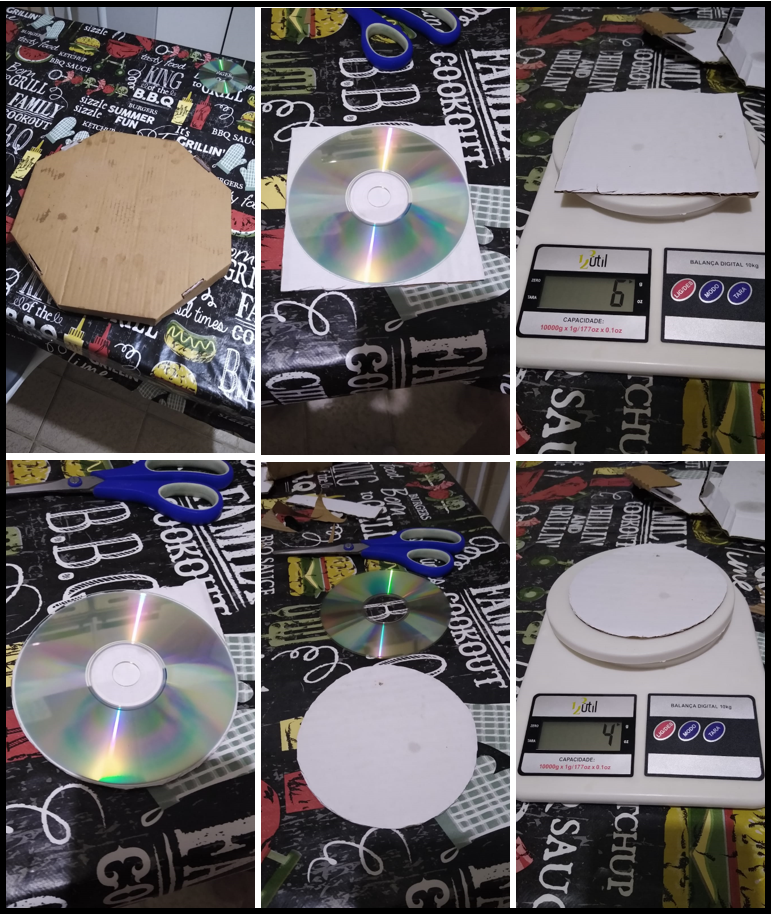
\includegraphics[width=0.7\linewidth]{PROGRAMACAO/pic/educacao/processo_01}
	\caption[]{Processo de construção dos objetos para a determinação da massa do quadrado e do círculo}
	\label{fig:processo01}
\end{figure}

Substituindo os valores na relação de $\pi$, tem-se:

\begin{ceqn}
	\begin{align*}
	\pi &= \frac{12 \cdot 12 \cdot 4}{6 \cdot 6^2} \\
	\pi &= \frac{144 \cdot 4}{216} \\
	\pi &= \frac{576}{216} \\
	\pi &= 2,666... \\
	\end{align*}
\end{ceqn}

Bom, claramente o valor que sabemmos sobre $\pi$ não é esse, mas \textit{onde está o erro?} A metodologia utilizada parece ser coerente e era de esperar uma diferença, pequena, mas poderia existir. Então, deve-se contentar com este resultado ou investigar mais? Obviamente que a investigação deve continuar e isso faz parte do processo; não basta apenas determinar uma metodologia e quando chegar no resultado final, OK, para! O resultado tem que ter SIGNIFICADO!

Uma possibilidade de investigação para ter um erro tão grande assim, está relacionada a \textit{precisão da balança}. 

Todo equipamento possui uma \textit{precisão}, ou seja, os equipamentos conseguem efetuar operações até um certo limite, após esse limite, os resultados não podem ser considerados.

A balança utilizada foi uma balança de cozinha que tem a capacidade de medir massas de até $10 kg$ com a unidade mínima em \textit{grama}, ou seja, ela consegue medir de 1 em 1 grama até 10 kg; Essa precisão não pode ser negligenciada dependendo do tamanho da massa que se mede, pois se medir algo que tenha 500 g, a forma correta de representação, nesse caso, seria $500 \pm 1 \text{g}$, sendo assim, esse objeto pode ter entre 499 e 501 grama. 

Os objetos do experimento possuem 6 g e 4 g, e através da balança utilizada, a medição pode ser 5-7 g e 3-5 g. Se dividir a precisão 1 g pela massa dos objetos tem-se: 0,17 ($\approx 16.7\%$) e 0,25 ($\approx 25 \%$), ou seja, a precisão da balança está na mesma \textit{Ordem de grandeza} da medida das massas dos objetos. Solução? Fazer mais quadrados e mais círculos com os mesmos tamanhos dos anteriores para que a precisão da balança fique em uma ordem de grandeza menor. As novas medições podem ser vistas na figura abaixo:

\begin{figure}[H]
	\centering
	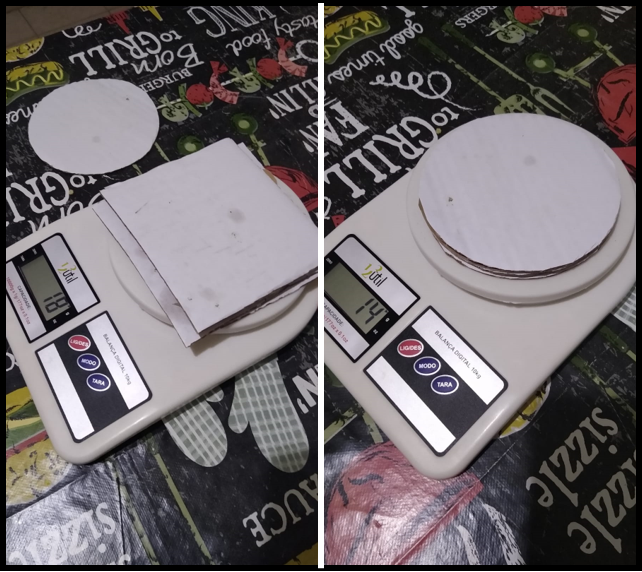
\includegraphics[width=0.7\linewidth]{PROGRAMACAO/pic/educacao/processo_02}
	\caption[]{Novas medições das massas.}
	\label{fig:processo02}
\end{figure}

Com essas novas medidas, a precisão da balança representa, apenas, $7,1\%$ da massa dos círculos e $5,6\%$ da massa dos quadrados. Assim, usando esses novos valores para as massas na relação montada para a determinação do $\pi$, tem-se:

\begin{ceqn}
	\begin{align*}
	\pi &= \frac{12 \cdot 12 \cdot 14}{18 \cdot 6^2} \\
	\pi &= \frac{144 \cdot 14}{18 \cdot 36} \\
	\pi &= \frac{2016}{648} \\
	\pi &= 3,111... \\
	\end{align*}
\end{ceqn}


Esse valor calculado representa muito bem o valor de $\pi$. O erro relacionado a este cálculo é de $0,9\%$. \textit{É possível melhorar o resultado?} Sim, é possível, usando uma balança de precisão, materiais de maior qualidade e homogêneos mas, para um processo de ensino-aprendizagem esse valor é surpreendente! Não pelo fato de ter calculado o valor aproximado, mas a quantidade de outros conhecimentos que podem ser discutidos.

\begin{exercise}
	Após a leitura desse texto, elabora um texto curto descrevendo o seu entendimento sobre Tecnologia.
\end{exercise}

\begin{exercise}
	A metodologia usada para a determinação do número $\pi$ experimentalmente possui uma quantidade de conhecimentos extras, ou seja, fora da exclusividade da matemática que podem ser explorados. Qual(is) desse(s) conhecimento(s) você nunca ouviu falar ou, foi extremamente diferente?
\end{exercise}

\begin{exercise}
	O tema do capítulo desse "futuro livro" está relacionado a \textit{softwares} mas, onde está a \textit{utilização do software}? Qual a relação desse tópico com a disciplina? 
\end{exercise}

\section{\textit{Softwares}}\index{\textit{Softwares}}

Muitos problemas na matemática podem ser resolvidos de \textit{modo analítico}, ou seja, sua solução pode ser calculada algebricamente, ou podem ser resolvidos de modo \textit{numérico}. Devido ao avanço da tecnologia, os computadores e, consequentemente, os \textit{softwares} permitem também cálculos algébricos.

Os matemáticos estão acostumados com algumas linguagens de programação e/ou softwares
%\chapterimage{chapter_head_2.pdf} % Chapter heading image

\chapter{Introdução ao Python}

\section{Conceitos iniciais}\index{Conceitos iniciais}
Nesta seção trabalharemos com o Python 3.x.
%\part{Bibliografia}						% <- Bibliografia
%\nocite{flemming2007,hoffmann2008,tan2008,jacques2010,bonafini2011,murolo2011,oliveira2016,barbosa2017,castanheira2017,panonceli2017,souza2018,munaretto2018,boldrini1986,steinbruch2009,franco2016,fernandes2017,domingues2018}

%----------------------------------------------------------------------------------------
%	BIBLIOGRAPHY
%----------------------------------------------------------------------------------------
\chapterimage{chapter_head_1.pdf} % Chapter heading image
\chapter*{Bibliografia}
\addcontentsline{toc}{chapter}{\textcolor{blue}{Bibliografia}} % Add a Bibliography heading to the table of contents

%------------------------------------------------

\section*{Artigos}
\addcontentsline{toc}{section}{Artigos}
\printbibliography[heading=bibempty,type=article]

%------------------------------------------------

\section*{Livros}
\addcontentsline{toc}{section}{Livros}
\printbibliography[heading=bibempty,type=book]

%%----------------------------------------------------------------------------------------
%	INDEX
%----------------------------------------------------------------------------------------

%\cleardoublepage % Make sure the index starts on an odd (right side) page
%\phantomsection
%\setlength{\columnsep}{0.75cm} % Space between the 2 columns of the index
%\addcontentsline{toc}{chapter}{\textcolor{blue}{Índice}} % Add an Index heading to the table of contents
%\printindex % Output the index

%----------------------------------------------------------------------------------------

\end{document}
